\documentclass[a4paper,twoside,12pt]{book}
\usepackage[utf8]{inputenc}
\usepackage{listings}
\usepackage{amsmath}
\usepackage{amsthm}
\usepackage{amsfonts}
\usepackage{amssymb}
\usepackage[english]{babel}
\usepackage[a4paper]{geometry}
\usepackage{graphicx}
\usepackage{epigraph}
\usepackage{color,psfrag}
\usepackage{fancyhdr}
\usepackage{makeidx}
\usepackage{mathpazo}
\usepackage{mathrsfs}
\usepackage{float}
\usepackage{datetime}
\usepackage{titlesec}
\usepackage{datetime}
\usepackage{afterpage}
\usepackage{pdflscape}
\usepackage{ragged2e}
\usepackage{adjustbox}
\usepackage{algorithm}%new
% \usepackage{algorithmicx}%new
\usepackage[noend]{algpseudocode}%new
\sloppy

%\usepackage{hyperref}
%\usepackage[numbers]{natbib}
\usepackage[labelfont=bf,textfont=it,labelsep=period,width=\textwidth]{caption}
\usepackage[unicode,pdfstartview={XYZ null null 1},pdfview={XYZ null null 1},pdfpagemode=UseOutlines]{hyperref}
\usepackage{booktabs}
\usepackage{graphicx}
\newcommand{\ra}[1]{\renewcommand{\arraystretch}{#1}}
\newcommand\blankpage{%
    \null
    \thispagestyle{empty}%
    \addtocounter{page}{-1}%
    \newpage}
\newdateformat{monthyeardate}{%
  \monthname[\THEMONTH], \THEYEAR}


\definecolor{szin}{rgb}{0.679,0.19,0.21}
\definecolor{szin2}{rgb}{0,0.445,0.734}
\definecolor{szin3}{rgb}{0,0.5,0}

\makeatletter
\let\stdl@chapter\l@chapter
\renewcommand*{\l@chapter}[2]{%
  \stdl@chapter{\textcolor{szin}{#1}}{\textcolor{szin}{#2}}}
\makeatother

%fejlï¿œc
\pagestyle{fancy}
\setlength{\headheight}{15.71667pt}
\lhead{\nouppercase{\rightmark}}
%\rhead{\nouppercase{\leftmark}}
\fancyhead[LE,RO]{\thepage}
\fancyfoot{}

%margomï¿œretek
\setlength{\marginparwidth}{0pt}
\setlength{\marginparsep}{0pt}
\setlength{\marginparpush}{0pt}
\setlength{\oddsidemargin}{24.1pt}
\setlength{\evensidemargin}{1pt}
\setlength{\footskip}{20pt}
\setlength{\headheight}{27.5pt}
    
%chapterstyles
\newcommand{\PreContentTitleFormat}{\titleformat{\chapter}[display]{\scshape\Large}
{\Large\filleft\MakeUppercase{\chaptertitlename} \Huge\thechapter}
{1ex}
{}
[\vspace{1ex}\titlerule]}
\newcommand{\ContentTitleFormat}{\titleformat{\chapter}[display]{\scshape\color{black}\huge}
{\color{szin}\Large\filleft\MakeUppercase{\chaptertitlename} \Huge\thechapter}
{1ex}
{\titlerule\vspace{1ex}\filright}
[\vspace{1ex}\titlerule]}
\newcommand{\PostContentTitleFormat}{\PreContentTitleFormat}
\PreContentTitleFormat


\begin{document}

\begin{titlepage}
	\begin{center}

		\textbf{\LARGE{Multilayer network analysis of sustainable, multimodal urban transport networks}}\\[3.3cm] %

		
\includegraphics[width=3.45cm,height=2.3cm]{images/ceulogo.eps}\\[3.4cm]
		{\Large{\textbf{Luis Guillermo Natera Orozco}}}\\[0.4cm]

		\medskip

		Department of Network and Data Science \\
		Central European University\\ [1.2cm]

		Supervisor: Federico Battiston \\
		External Supervisor: Michael Szell

		\vfill

		A Dissertation Submitted in Partial Fulfillment of the Requirements\\ for the Degree of Doctor of Philosophy in Network Science\\[2cm]

		%
\includegraphics[width=3cm,height=2cm]{images/ceulogo.eps}\\[0.5cm]
		% Central European University\\
		% Budapest, Hungary

		\vspace{1.0cm}
		\the\year
	\end{center}
\end{titlepage}

\newpage

\pagestyle{empty}

\mbox{}

\vfill

\noindent Luis Guillermo Natera Orozco: \emph{Multimodality and sustainability in urban networks}, \copyright \\
\the\year \\ All rights reserved.



\mbox{}

\pagestyle{empty}

\newpage


\chapter*{Researcher declaration}
I Luis Guillermo Natera Orozco certify that I am the author of the work Multimodality and sustainability in urban networks. I certify that this is solely my own original work, other than where I have clearly indicated, in this declaration and in the thesis, the contributions of others. The thesis contains no materials accepted for any other degrees in any other institutions.  The copyright of this work rests with its author. Quotation from it is permitted, provided that full acknowledgement is made. This work may not be reproduced without my prior written consent.

\subsection*{Statement of inclusion of joint work}
I confirm that Chapter~\ref{ch:litReview} is based on a paper wich was written in collaboration with Laura Alessandretti, Michael Szell and Federico Battiston. Dr. Battiston and I concived the idea of doing a review about the application of multiplex networks to the study of urban mobility systems. All authors contributed to the writing of the paper. Dr. Battiston endorses this statement with his signature below.

\vspace{.2cm}

I confirm that Chapter~\ref{ch:OverlapCensus} is based on a paper wich was written in collaboration with Federico Battiston, Gerardo I\~niguez, and Michael Szell. I, with Dr. Battiston and Dr. Szell concived the idea of the overlap census. I collected the data and carried out the analyses. All authors developed the methods used, contributed to the writing of the paper on which the chapter is based and gave final approval for publication. Dr. Szell endorses this statement with his signature below.

\vspace{.2cm}

I confirm that Chapter~\ref{ch:BikeGrowth} is based on a paper wich was written in collaboration with Federico Battiston, Gerardo I\~niguez, and Michael Szell. I, with Dr. Battiston and Dr. Szell concived the research. I collected, processed and cleaned data, and carried out the computational analysis. All authors designed the algorithms, analysed the data and results, and helped draft the manuscript. Dr. Szell endorses this statement with his signature below.

\vspace{.2cm}

\noindent
I confirm that Chapter~\ref{ch:LQI} is based on a paper wich was written in collaboration with D\'avid Deritei, Anna Vancs\'o, and Orsolya V\'as\'arhelyi. I with Dr. Deritei and Dr. V\'as\'arhelyi concived the research and methodology, all authors collected, processed and cleaned data, and carried out the computational analysis. Together with Dr. Deritei and Dr. V\'as\'arhelyi we analyzed the results. All author helped draft the manuscript and gave final approvement for its publication. Dr. V\'as\'arhelyi endorses this statement with her signature below.

\vspace{0.5cm}
\noindent
Signature of PhD Candidate:

\vspace{2cm}
\noindent
\monthyeardate\today


\vspace{3.5cm}
\noindent
Signature of Dr. Federico Battiston, endorsing statement of joint work:

\vspace{2cm}
\noindent
\monthyeardate\today


\vspace{3.5cm}
\noindent
Signature of Dr. Michael Szell, endorsing statement of joint work:

\vspace{2cm}
\noindent
\monthyeardate\today

\vspace{3.5cm}
\noindent
Signature of Dr. Orsyola V\'as\'arhelyi , endorsing statement of joint work:

\vspace{2cm}
\noindent
\monthyeardate\today




\chapter*{Abstract}
In this thesis, we use network science to study cities and their mobility infrastructures. We treat these infrastructures as layers of a multiplex network, such as sidewalks, bicycle paths, subway systems and streets, and develop and apply network science based tools to study these layers both individually and jointly.\\

First, we cover the existing literature of cities as multiplex networks, from infrastructure and dynamics to existing measures, data and analysis tools. Second, we propose a new method to extract the multimodal profile from a city's multiplex transport network. We show how this method can be applied to identify multimodal similarities between cities. Third, we focus on the bicycle layer of the multimodal network, investigate its structure, and find that it consists of hundreds of disconnected patches. To connect these patches, we develop and apply data-driven, algorithmic network growth strategies, showing that small but focused investments allow to significantly increase the connectedness and directness of urban bicycle networks. In the forth chapter, we present a data-driven, network-based method to quantify the liveability of a city, computing pedestrian accessibility to amenities and services, taking into consideration safety and environmental variables. Finally, we discuss the main contributions of this thesis and outline possible applications and open questions for the future.

\thispagestyle{empty}

\chapter*{Acknowledgements}
\textcolor{red}{To be written}



\thispagestyle{empty}

\newpage
\frontmatter

\pagestyle{fancy}

\newpage
\addcontentsline{toc}{chapter}{Contents}

\PreContentTitleFormat

\def\luis#1{{\small\color{red}\textbf{[Luis: #1]}}}

\tableofcontents

\PreContentTitleFormat

\newpage

\PreContentTitleFormat

\pagestyle{fancy}

\newpage
\PreContentTitleFormat
\pagestyle{fancy}

% \listoftables
% \addcontentsline{toc}{chapter}{List of Tables}

% \listoffigures
% \addcontentsline{toc}{chapter}{List of Figures}

\PreContentTitleFormat
\newpage
\mainmatter
\ContentTitleFormat

\chapter{Introduction: Cities and networks}
%Why study cities? 

\epigraph{Cities have the capability of providing something for everybody, only because, and only when, they are created by everybody.}{Jane Jacobs, \textit{The Death and Life of Great American Cities} (1961, p. 238)}

As a complex system, a city offers a fertile study ground from multiple perspectives. Urban studies, from sociological perspectives to more technical ones such as engineering, have engaged in analyzing different aspects of urban life. Due to this diversity and overlapping approaches, the ``science of cities'' is inherently interdisciplinary.

\textcolor{red}{In cities, interdisciplinary goes beyond the application of tools and methods borrowed from one discipline, and their application to study a different object. Indeed, when we think and engage in the analysis of urban phenomena, we encounter a multitude of approaches without a single dominant one. When studying cities one can start taking apart its pieces and analyze them separately. Take for example buildings, roads, and functions, all of them can be study without taking into consideration the rest of the pieces. However, following this approach misses the interactions between the pieces. Thus, to have a complete view of those interactions, and a better understanding of cities, we can study them as a system. To do so, we can use networks.}

\section{From architecture to network science, a personal journey}

As an architect my first approach to study cities was from the buildings' perspective, understanding how, by building, we delimit and shape spaces that model experiences in the city~\cite{gehl1971life}. These buildings are fundamental to define public spaces, mobility infrastructures, and even services that enable us to inhabit the \textit{ville}~\cite{sennett2018building}. The way we shape the city has an influence in how we inhabit it. Thus, understanding its infrastructures is fundamental to understand and plan better cities for an increasingly complex future. Especially, when tackling urban mobility challenges, the way we plan, build and use mobility infrastructures is fundamentally entangled with the livability of our cities.

\textcolor{red}{When thinking about urban infrastructures, my first approach was to use drawings and blueprints. These tools are useful to understand, and plan urban mobility. They provide a way to move from the physical structure of cities, to a more concrete way to represent them. These maps and blueprints provide a useful way to abstract the reality and make it more manageable. Of course, one has to be cautious when building such maps, at the end they are a representation of the territory, not the territory itself~\cite{borges1961hacedor}.}

%Talk about curiosity, why study cities from the complex systems perspective, and specially from network science.
After working in designing public policies to promote bicycle infrastructure in my home-city's government, I became interested in getting to understand the relation between different transportation modes, and how cities and their mobility infrastructures could be studied using large scale data systematically. This curiosity led me to the complex systems field, and the use of network science to study cities.

\luis{write more about moving between architeture and network science.}
\begin{itemize}
    \item Public spaces
    \item Urban mobility
    \item Complexity, cities as fractals (Batty)
    \item The always evolving city. We cannot predict the future, we can build it. Tools to understand the present and build a sustainable future.
    \item Personal reflection of interdisciplinary approaches (social sciences benefit from quantitative methods, but it is important to acknowledge interdisciplinary as a two-way street, recognize the importance of social sciences, and the long tradition of urban studies. Not because we have a hammer, should we treat everything as if it were a nail) \luis{This idea might go to conclusions.}
\end{itemize}
% While predicting how the future city will be is an impossible task, understanding how it has evolve and what is its state of development is possible. This understanding 


\section{Aim and structure of the thesis}

\luis{I still have to write about the thesis, from where does it start (complex systems and the study of cities) to the main contributions. I anticipate two paragraphs for the complex systems and cities, and two more paragraphs for the contributions/overview.}

The primary aim of this thesis is to contribute to the better understanding of the structural properties of multimodal transportation networks in urban areas. For that, we build on the tools and methods of network science to analyze the underlying complexity of urban mobility infrastructure. 

In the first part of this thesis we focus the attention on the multimodal infrastructure networks, first providing a review of previous works, and then giving an original contribution to the analysis of multilayer transportation networks. In the second part, we focus the attention to specific layers, first bicycle, then pedestrian infrastructure.

This thesis is structured as follows:

\begin{itemize}
    \item Chapter~\ref{ch:litReview}: We provide a review of previous works on multimodal transportation and mobility research from a complex systems' perspective. First we focus on the infrastructure and measures to quantify it, then on the mobility dynamics on top of these infrastructures, and finally we offer a review of available datasets and tools to analyze this specific type of networks.
    \item Chapter~\ref{ch:OverlapCensus}: We make an original contribution to the field by proposing a method to extract the multimodal profile from a city's multiplex transport network. We apply our methods to fifteen cities, finding clusters of cities with similar multimodal infrastructure.
    \item Chapter~\ref{ch:BikeGrowth}: We focus our attention in the bicycle layer of the multimodal network and propose algorithmic approaches to improve its connectivity. We find that focalized investment has the potential to rapidly improve the connectedness and directness of the bicycle infrastructure.
    \item Chapter~\ref{ch:LQI}: We present a methodology to measure the quality of life in a city based on the pedestrian accessibility to amenities and services. We apply the methodology to Budapest and show how it can be used to capture inequalities in neighborhoods. 
    \item Chapter~\ref{ch:Conclusion}: We review the main contributions from this thesis, and outline future streams of work and open questions. 
\end{itemize}\pagestyle{fancy} %Introduction
\chapter{Related Work: Multimodal transportation and mobility in urban networks}\label{ch:litReview}

In this chapter we provide a comprehensive overview of complex systems approaches to multimodal transportation and mobility in urban networks. We cover multiple approaches that had been used to model cities using the multiplex framework, measures to quantify centralities and changes in the given networks and layers. After reviewing the mobility infrastructure and measures, we move our focus to the mobility dynamics on top of those layers, covering the study of urban mobility dynamics in public transport systems and at individual level. Finally, we conclude the chapter with an overview of the available data and computational tools for the study of urban mobility networks\footnote{A stand alone of this chapter is currently being prepared as a paper, to be submitted to Transportation Reviews. No preprint is yet available.}.

% \section{Cities as complex systems}
% In this first chapter we offer a comprehensive review of multimodal transportation and mobility research focusing on recent complex systems approaches. In such approaches, the city is studied as a complex system \cite{batty2013new,lobo2020urban}, in which especially urban transport infrastructure, such as streets, sidewalks, bicycle lanes and public transportation systems can be well modelled and understood using methods from network science. From this perspective, single-layer spatial networks, especially transportation networks, have been widely studied~\cite{lin2013complex,barthelemy2011spatial,ding2019application}, finding different topological properties~\cite{jiang2004topological,cardillo2006structural,barthelemy2008patterns,batty2008size,barthelemy2011spatial,strano2013comparative,louf2014typology,boeing2020multiscale}, distribution of centrality metrics~\cite{crucitti2008centrality,Boeing2020Planarity,kirkley2018structural}, and network growth processes~\cite{makse1995growth,strano2012evolution}. Further topics studied include impacts of the street networks on pedestrian volume \cite{hajrasouliha2015connectivity}, accessibility and vitality of cities~\cite{denadai2016death,biazzo2019accesibility,natera2020walkability}, and resilience and growth of different transportation networks~\cite{baggag2018resilience,ferretti2019resilience,natera2020growth}. %Despite the many successes, network science should be applied to transportation systems with care \cite{zanin2018studying}. 

% The most recent of these approaches can be seen as the beginning of the emerging field of Urban Data Science, which exploits large-scale new urban data sets with tools combining geoinformatics, data and network science \cite{organizers2019roundtable,resch2019hds}.

In this chapter, we survey the literature on urban multimodal mobility, and on urban transportation infrastructure as multilayer networks. Here, we focus on the primal approach to networks~\cite{porta2006primal}, where streets and mobility infrastructure constitute the network links, and intersections (bus stops, subway stations, etc.) constitute the nodes of the network.

The remainder of this chapter is arranged as follows. Section~\ref{sec:multilayernetworks} introduces the mathematical concept of multilayer networks and related theoretical research underlying network science approaches to the topic. In Section~\ref{sec:multimodalinfrastructures} we discuss research on urban transport infrastructures, including their theoretical modelling (see Subsection \ref{sec:multimodalinfrastructures}) as multilayer networks and their empirical characterization (see Subsection \ref{sec:measuresinfrastructure}). In Section~\ref{sec:multimodalmobility} we focus on mobility, flows and navigation across these multimodal systems, and implications for transportation choices. In Section ~\ref{sec:datatools} we cover the relevant open datasets and the main software tools which can be used to analyse multimodal transportation systems. %We conclude with an outlook and a summary of open questions for the research community in Section~\ref{sec:conclusions}. 

\section{Multilayer networks: A framework for multimodality}\label{sec:multilayernetworks}

Over the last decades, networks have emerged as a versatile tool to understand, map and visualize the interconnected architecture of a wide range of complex systems~\cite{albert2002statistical,dorogovtsev2002evolution, newman2003structure, boccaletti2006complex}, in particular spatially-embedded ones~\cite{barthelemy2011spatial, barthelemy2018morphogenesis}. Formally, a network -- or graph -- $\mathcal G = (\mathcal N, \mathcal L)$ consists of a set of nodes $\mathcal N$, and a second set $\mathcal L$ of edges, describing connections among unordered pairs of elements of the first set. This information can be conveniently stored into an adjacency matrix ${A=a_{ij}}$, where $i=1, \dots, N$ are the nodes, and $a_{ij}=1$ if there is a link between nodes $i$ and $j$, $a_{ij}=0$ if there is no link between $i$ and $j$. In transportation systems~\cite{lin2013complex}, nodes can represent the stations of a network, and links direct connections between them. The adjacency matrix can also include weights $W=w_{ij}$, where $w_{ij}$ are positive real numbers, for instance describing how strongly connected two nodes are. For spatial systems, weights are often taken as the reciprocal of the distance between two nodes, or the time it takes to travel from one to another, i.e. $w_{ij}=1/d_{ij}$ or $w_{ij}=1/t_{ij}$.

More recently, network scientists have put effort into characterizing the structure of systems which are formed by different interconnected networks. Such interconnected structures are natural for transportation systems but also for social and biological networks. Think for instance of the largest transportation hubs in worldwide cities, where stations are routinely served by bus, underground and railway infrastructures.

Indeed, most urban transportation systems systemically rely on the interplay between different means of transportation. These systems can be conveniently described by \textit{multiplex} or \textit{multilayer} networks. Here we introduce the \textit{vectorial} formalism for multilayer networks~\cite{boccaletti2014structure, battiston2014structural}, widely used in most papers on multimodal transportation. An alternative description can be provided by a more mathematically involved \textit{tensorial} framework~\cite{dedomenico2013mathematical, kivela2014multilayer}.  

In multilayer networks, links of different types, describing for instance a different mean of transportation, are embedded into different \textit{layers}. Each layer $\alpha$, $\alpha = 1, \ldots, M$, is described by an adjacency matrix $W^{[\alpha]} = \{w_{ij}^{[\alpha]}\}$. In a multimodal urban transportation network with three mobility infrastructure layers, $\alpha=1$ can represent the bus network, $\alpha=2$ the underground network, and $\alpha=3$ the urban railway network, for example. The full transportation system $\mathcal M$ can be described as $\mathcal W = \{ W^{[1]}, \ldots,  W^{[M]}\}$. Nodes $i=1, \dots, N$ are labeled in the same order in all networks. 

In the case of transportation networks, simply identifying nodes of different networks as the same station might not provide the most complete description of the multimodal network. Take for instance the largest stations in mega-cities, like King's Cross - St. Pancras in London, Grand Central Station in New York or Hongqiao transportation hub in Shanghai. All of these are identified by a unique location (node index) $i$ across the different transportation layers. Yet, switching from one mean of transportation to another within the same station might require a non-negligible fraction of time and effort, given the complexity and size of the overall infrastructure. 

For this reason, it is often relevant to complement the description of the \textit{intra-layer} connections present in the system, with \textit{inter-layer} links associated to the cost, spatial distance or time required to switch layers. Inter-layer links between layers $\alpha$ and $\beta$ at a node $i$ can be encoded through the inter-layer matrix $C_i=\{c_i^{[\alpha \beta]} \}$, and all such inter-layer connections can be stored in the vector $ C = {C_1, \ldots, C_N}$. In this case, the full multiplex structure of the system is described by taking into account both intra-layer and inter-layer connectivity, hence $\mathcal M = ( W,  C)$. Inter-layer links may be neglected for many measures focusing on diversity~\cite{battiston2014structural}, as well as correlations~\cite{nicosia2015measuring} across the layers of the systems, relevant to assess the different roles and geographical spanning of the different mean of transportations of a multilayer network. 

Multilayer networks are a natural framework for multimodal transport networks. Indeed, one of the pioneering works introducing the framework and concept of ``layered complex networks''~\cite{kurant2006layered} explicitly focuses on the case of transportation systems, where a first layer encodes the physical infrastructure of the system, and the second one describes the flows on such infrastructure. Other early works on the topic also dealt with interconnected systems at the worldwide level, focusing on different modes of transport such as the multiplex airline networks~\cite{cardillo2013emergence}.

Noticeably, multimodal infrastructures seem to possess exclusive characteristics different from other multilayer networks. For instance, when tools to assess the redundancy of the different layers are considered, transportation networks are often found to be irreducible~\cite{dedomenico2015structural}. Differently from many biological systems, where layers often duplicate information to guarantee the interconnected system a high level of robustness, the layers of a multiplex transportation systems are purposedly engineered to be different, in order to maximise efficiency~\cite{latora2001efficient}. As a byproduct of this feature, multimodal systems are also often highly fragile~\cite{buldyrev2010catastrophic}, and sensitive to disruptions or failures of a single infrastructure~\cite{dedomenico2014interconnected}. For the reader interested in further material on the topic, we refer to the early reviews~\cite{boccaletti2014structure, kivela2014multilayer} and textbook~\cite{bianconi2018multilayer} covering the field. Aleta et al.~\cite{aleta2019multilayer} provides a more recent eye-bird view of the field. A thorough review of the measures and models used to analyse such systems can be found in Battiston et al.~\cite{battiston2017new}, whereas de Domenico et al.~\cite{dedomenico2016physics} gives a theoretical overview of spreading and diffusive processes on such systems. In the following sections of this chapter, we focus on findings of more direct relevance to the research community working with multimodal transportation and urban mobility. The division of related research across these two themes is not meant to be rigid, but rather serves as an indication of the core topic treated in the different works. 


\section{Multimodal infrastructures}\label{sec:multimodalinfrastructures}

As cities grow and add different transportation modes, understanding the transportation infrastructure and its interconnected nature is crucial to capture patterns of urban mobility. Since the 1950s, fields ranging from Architecture to Urbanism and Transport Planning have grown a large body of literature studying the structure of cities and their transport systems. With the growth of the Complex Systems and Network Science fields, new models have been developed to study the complexity behind urban systems, and specifically mobility infrastructure.

Multimodal urban infrastructures can be represented as multilayer networks, in which each layer $\alpha$ represents a mobility infrastructure (e.g. subway, light railway, bus service, pedestrian or bicycle infrastructure), the set of nodes $\mathcal{N}$ are locations (e.g. bus stops, intersections, subway stations), and the set of edges $\mathcal{L}$ in layer $\alpha$ are the infrastructure links between nodes in the same layer (e.g. subway lines, bus routes, bicycle lanes, see also Section \ref{sec:multilayernetworks}). Modeling infrastructures is of great importance for understanding how urban systems work, and for the design of new sustainable mobility options. 

In the following we describe recent findings related to how transportation layers are coupled and grow. First, we review the main complex systems models of urban transportation. Then, we describe empirical findings related to the transport infrastructures.

\subsection{Modeling urban infrastructure}\label{sec:modelinginsrastructure}

One of the first contributions to the modeling of multimodal urban infrastructures was provided by de Cea et al.~\cite{decea2005equilibrium} who pointed out that most of the models from the transport community~\cite{boyce1994introducing,boyce2002sequential,decea2007} used to plan and simulate the effects of new transportation options and failed to consider congestion associated with transit modes. This shortcoming is particularly relevant when the models are used for infrastructure development and predict transportation equilibria in future years. 

The model proposed by de Cea et al.~\cite{decea2005equilibrium} takes the road network as the base layer. There, links have an average operating cost that takes into account different mobility options (e.g. cars, taxi, etc.). For every public transportation mode a new layer is defined, with their unique nodes and links. For these layers, the cost function of the public transportation links depends on the combined effect of travel, waiting, and transfer time. The model considers the existence of combined trips (e.g. car/metro, bus/metro, etc) and looks for an equilibrium condition under the assumption that every user chooses her route to minimize their average operation cost (Wardrop’s first principle). This means that at equilibrium, only non-congested routes have a minimum cost, while those without flow represent a more costly option. Travel time might be affected by the interplay of different transportation means. For instance, vehicle flow over the road network may induce longer travel times in the bus network. Similarly, a passenger might decide not to take the subway if it is too crowded. \cite{decea2005equilibrium} show that their model is able to find the equilibrium in the trips between origin and destination in a toy model, and can be successfully applied to real-world scenarios. For instance, a rich version of this model (which consisted of 13 user classes, 11 transport modes, and 450 zones) successfully informed the planning of the new metro line 5 in Santiago (Chile).

A similar philosophy was deployed by Li et al.~\cite{li2007parkride} who considered a transportation infrastructure of cars, combined walk-metro paths, and park-and-ride. Differently from the previous work in which the model takes in consideration the availability of routes, here parking availability and time spent by car commuters while looking for parking, which can be considerable~\cite{shoup2017high}, is considered explicitly. The focus here is on the interplay and impact of park-and-ride (P\&R) schemes to encourage users to switch from car travel to subway and public transportation options when traveling to the cities' central area. The model proposed by Li et al.~\cite{li2007parkride} considers the effects of traffic conditions on travel demand, and incorporates elastic demand into the model to capture commuters’ responses to traffic congestion and availability of parking supply. The responses of a user include the decision to switch to another transportation option, or to not make the trip at all. For the public transportation layer, the model also takes in consideration discomfort that may result from crowded subways. Through numerical simulations, Li et al.~\cite{li2007parkride} found that it is possible to reach an equilibrium control which prevents the emergence of traffic jams in the city center by implementing a suitable P\&R scheme, which looks at the combined effect of cost at the P\&R sites, parking availability in the city center, as well as metro fares and frequency.

While in the above works the interplay of different transportation modes was introduced, they were not yet  modeled as a multilayer network. One of the first applications of this new modeling framework was presented by Morris et al.~\cite{morris2012transport} who developed a toy model to couple different transport modes, according to the following rules. First, \textit{N} nodes are placed at random within the unit circle, mimicking a spatial configuration typical of many cities, and are connected by a Delaunay triangulation. Second, to simulate another transport mode, a second layer is generated by drawing a subset of the previously generated nodes and a second Delaunay triangulation. Finally, the two layers are coupled with interlayer links when a node is present in both layers. Using this toy model and a simulated Origin-Destination matrix, Morris et al.~\cite{morris2012transport} investigated how fragile the network is to changes in supply and demand. They found that increasing travel speed in one layer tends to concentrate trips in the fastest layer, and also produces congestion in the nodes where is possible to change transport mode.

Similar results have been reported for coupled random networks~\cite{gao2017comprehensive}, as well as scale-free networks~\cite{zhuo2011traffic} where a similar modelling approach is used to mimic a real-world transport scenario~\cite{du2016physics}. In their work, Du et al.~\cite{du2016physics} used a two-layer traffic model, where one layer provides higher transport speed than the other, and applied a Particle Swarm Optimisation algorithm to optimize the transport system capacity and reduce congestion both in synthetic and real-world multimodal networks. A more detailed coverage of the findings can be found when discussing betweenness centrality and interdependence in Section~\ref{sec:measuresinfrastructure}. 

Gil~\cite{gil2014configuration} proposed to use open data from Open Street Map to model the multimodal infrastructure network of a given city as a combination of three layers. The first layer is the street network, where the nodes are intersections and links are streets. This layer, accounting for private transportation, was again the reference layer with respect to the other transportation modes in the system, i.e.~all other layers have to be connected to and interact with it. The second layer is the public transport layer that represents the stations as nodes. It links the stations whenever there is a public transport service between two stations. This layer is coupled to the street layer by the stations and their closest street intersection. Gil~\cite{gil2014configuration} also include in their model land use to measure urban accessibility. This framework was applied to the analysis of the Randstad city-region in the Netherlands. The model was tested under different parameters and layer combinations, measuring reachability of the different city areas through closeness and betweenness centralities. Comparison with ground truth data showed that betweeness centrality in the public transportation layer can be a good indicator of passenger flows.

Aleta et al.~\cite{Aleta2017Multilayer} exploited one step further the richness of multilayer networks for transportation systems, highlighting two possible frameworks. In the first framework, each bus or metro line on its own could be considered an independent layer. This approach is useful to have a realistic model of human mobility which takes into consideration transfer times and synchronization between single trips. Yet, it does not allow to evaluate the importance of an entire transportation mode. This issue is resolved in the second framework. Here all the lines of the same mode are combined into a so-called \textit{superlayer}, which is fundamental to study the interdependence and resilience of the whole system. 

Using the previously described frameworks, Aleta et al. \cite{Aleta2017Multilayer} investigated the public transport systems of nine European cities. Following the first framework, the authors focused on some structural features of the emerging system such as the overlapping degree (sum of the node's degree in all layers~\cite{battiston2014structural}). They found that public transport infrastructures have some universal properties, and that the maximum overlapping degree is quite similar in all the systems, even if the number of layers is different. This depends on the fact that networks are embedded in a physical space, hence imposing some bounds on the maximum number of links of each node structural constraints. Following the second framework, Aleta et al.~\cite{Aleta2017Multilayer} investigated in detail the superlayers and found that -- suprisingly -- the nodes with the highest overlapping degree are not necessarily the ones with the highest superlayer activity~\cite{nicosia2015measuring} Indeed, some transportation modes (and in particular the bus layer) have a tendency for hubs which might be disconnected to the other transportation modes, leading to high overlapping degree but low multilayer activity. The prevalence of such hubs is relevant when considering the robustness of the whole system. As the study highlights, it is often easier to move a bus stop to a street nearby, even if it is a local hub where multiple lines stop, than solving a disruption in a subway station. Aleta et al.~\cite{Aleta2017Multilayer} also assess the importance of the superlayers based on the number of shortest paths that make use of the superlayer, a measure that we characterize later in Section~\ref{sec:measuresinfrastructure}.

It is important to note that cities and their transportation systems are not static in time. This means new transport modes may be introduced or extended, such as when new bus/subway stops are added. Recently, to plan for Open Streets during the COVID-19 pandemic, Rhoads et al.~\cite{rhoads2020planning} proposed an investigation of the relation between streets and sidewalks. First, the authors used percolation theory to examine whether the sidewalk infrastructure in cities can withstand the tight pandemic social distancing. They then proposed an algorithm that takes into consideration both the sidewalk and street layers while improving the sidewalk connectivity. Despite spatial constraints, Rhoads et al.~\cite{rhoads2020planning} showed that it is possible to widen the sidewalks and improve the pedestrian connectivity with a minimum loss in the road network. 

More in general, some works have focused on the growth and evolution of multilayer networks~\cite{nicosia2013growing,kim2013coevolution,nicosia2014nonlinear}, generalising preferential attachment mechanisms in different ways~\cite{barabasi1999emergence}. However, these works do not keep into account spatial constraints, and are not well suited to describe the evolution of spatial networks. For this reason, there is ample potential for future work to develop growth models for multimodal infrastructures, for instance considering densification and exploration, as previously done for street networks~\cite{strano2012evolution}. An alternative view can be obtained by investigating the optimal growth and design of the multiplex structure of the different layers, as was done for the multilayer airline network composed by routes of different airline companies~\cite{santoro2018pareto}. 

The models discussed in this section shown how the multilayer networks framework has been used to investigate the structure, function and vulnerabilities of a complex transportation system. In the next section we cover some measures to quantify the multiplexity of these structures and their interconnections.

\subsection{Characterizing multimodal infrastructure}\label{sec:measuresinfrastructure}

The empirical study of urban transportation infrastructure has revealed some of the structural properties of specific transport networks~\cite{barthelemy2011spatial}. But how to quantify the effectiveness of their interconnections? In this section, we describe a number of measures that have been used to capture the multiplexity of multimodal infrastructures, such as the importance of different nodes, the system's resilience, and the similarity between layers.

\paragraph*{Paths} 
At a more global scale, multimodality is often associated with the ability of an agent to navigate the system by using the available transportation modes. For this reason, the navigation of an agent in a transportation network can be measured through the available types of paths.

A first possibility is to consider the quickest path, neglecting transfer and waiting times between transportation modes. This path is computed using the fastest speed associated to the edges, assuming a perfect synchronization between the different transportation modes. This is analogous to finding the shortest path between $i$ and $j$ in an aggregated weighted-single layer network, where the weight describing the time to travel between two nodes is the minimum among those offered by the different transportation options.

Yet, this approach often falls short in capturing real patterns of mobility. Indeed, transportation networks also have a temporal dimension that has to be taken into consideration. In order to find a path that allows for a change between two or more different transportation options we must find a time-respecting path~\cite{Gallotti2014Efficiency}, defined as the shortest path between nodes $i$ and $j$ that considers the departures and arrivals constraints given by timetables. Such timetables are often shared by transport agencies using General Transit Feeds Specification (GTFS) Feeds; for an overview of possible data sources see Section~\ref{sec:datatools}. Furthermore, for multimodal transportation networks, the walking transfer time between modes has to be taken into account when computing time-respecting paths.

Besides time constraints, in order to find a viable path between $i$ and $j$, the logic of the proposed sequence of modes has to be assessed~\cite{battista1996path,lozano2001path}. For instance, in some cases, a path composed by subway-bus-subway-car-subway might solve the shortest path, but the presence of private transportation (car) as an intermediate option makes it an ``illogical path'' and thus an unlikely choice for a user. The validity of transportation sequences can in general be formalized in terms of cost associated to change of transportation mode.

Finding viable paths is one of the most important problems in urban transportation, as it has the potential to help users finding the most efficient paths in the city. Lozano et al.~\cite{lozano2001path} have proposed an efficient algorithm to find such paths when the agent establishes her limitations on the number of modal transfers.

The contribution of the different layers of a multiplex networks to shortest paths might be very unequal~\cite{Aleta2017Multilayer}. For instance, the rail systems (trams, subway) contribute to most of the shortest paths in a city, connecting distant points at a greater velocity and in straighter routes than bus or other transport modes. However, such layers have only few stations. Slower and more local transport modes often serve a complementary role, offering a deeper coverage of the city.

\paragraph*{Spatial outreach}
% The availability of different transportation modes, such as subways or tramways affects how easily it is to reach certain locations in the city. One possibility to measure this effect is to quantify the associated \textit{spatial outreach}. As defined in \cite{strano2015features}, the spatial outreach can be computed as the average Euclidean distance from node $i$ to all other nodes in the same layer $\alpha$ that are reachable within a given travel cost $\tau$. Mathematically it is defined as follows:
The availability of different transportation modes, such as subways or tramways affects how easily it is to reach certain locations in the city. A way to measure this effect is to quantify the associated \textit{spatial outreach}~\cite{strano2015features}. The spatial outreach can be computed as the average distance from node $i$ to all other nodes in the same layer $\alpha$ that are reachable within a given travel cost $\tau$. Mathematically it is defined as follows:

\begin{equation}
    L_\tau(i)=\frac{1}{N(\tau)}\sum_{j|\tau_{m}(i,j)<\tau}d_e(i,j),
    \label{eq:outreach}
\end{equation}

where $d_e(i,j)$ is the distance between nodes $i$ and $j$, and $N(\tau)$ is the number of nodes reachable on the multilayer network within a travel cost $\tau$.

Strano et al.~\cite{strano2015features} modified the average speed (traversal time of a link) in the layers of multiplex systems to measure their effects on the corresponding travel outreach. Strano et al.~\cite{strano2015features} found that when the metro speed increases compared to the street layer speed, a clear area of high-outreach nodes emerges in the city center and around the nodes that have connections to the high-speed layer. In other words, as the velocity in layer $\beta$ increases, the nodes that are closer to the interchange nodes in layer $\alpha$ improve their accessibility, implying that a person can efficiently travel from this area to faraway places. This concept of travel outreach is similar to that of isochrones which quantify the accessible area from a given point within a certain time threshold, e.g.: What is the area that a user can reach traveling $x$ minutes, in any direction, from a given point? Biazzo et al.~\cite{biazzo2019accesibility} used this approach to measure accessibility in different urban areas computing the isochrones as a combination of public transit and pedestrian infrastructure. With this method, scores were obtained that capture how well a city is served by the public transit and how accessible a specific area is to the rest of the city.


\paragraph*{Betweenness centrality and interdependence}
The relevance of the nodes in a network is characterized by centrality scores. Additional to single layer networks, in multiplex networks the overall centrality of a location or station also depends on the interplay of the different transportation options.

The simplest way to define the centrality of a node is to measure its degree, or the number of locations directly connected to it. Such a measure, however, is not so relevant for systems embedded in space due to spatial constraints. For example, the number of possible connections of a given node (intersection) in the street layer is highly constrained by the physical space, as a single intersection can only have a limited number of intersecting streets/sidewalks. For this reason, other centralities than degree are typically used to assess the relevance of a location. One of such measures is the betweenness centrality~\cite{Freeman1977Centrality}, measuring the number of shortest paths passing via a given node. This measure is also called ``load'' and can be seen as the simplest proxy for traffic flow in the system as it assumes uniform demand between each pair of nodes. In the absence of explicit mobility data, betweenness centrality can be used as a proxy to assess the areas at risk to become overcrowded and to identify potential bottlenecks in the system. 

In multiplex networks, shortest paths go from one node to another able to pass through two or more layers. This effect can be quantified by measuring the interdependence of a given node $i$ as:

\begin{equation}
    \lambda_i=\frac{1}{N-1}\sum_{j\neq i}\frac{\psi_{ij}}{\sigma_{ij}},
    \label{eq:coupling}
\end{equation}

where $\psi_{ij}$ is the number of shortest paths between $i$ and $j$ that use edges in two or more layers, and $\sigma_{ij}$ is the total number of shortest paths between $i$ and $j$~\cite{morris2012transport,battiston2014structural,strano2015features}. Node interdependence takes values in $[0, 1]$, with values close to 1 associated to a high coupling of the layers, while values close to $0$ mean that most of the paths from that node to other nodes go through just one layer. By taking the average over all nodes $\lambda = 1/N \sum_i\lambda_i$ it is possible to obtain a single score for the whole system. 

This interdependence measure can be modified to obtain a score for a specific layer~\cite{Aleta2017Multilayer}. Then the layer interdependence for layer $\alpha$ is defined as:

\begin{equation}\label{eq:layer_interdependency}
    \lambda^{\alpha}=\frac{\sum_i\sum_{i\neq j}\psi_{ij}^{\alpha}}{\sum_i\sum_{i\neq j}\psi_{ij}},
\end{equation}

where $\psi_{ij}^\alpha$ describes the number of shortest paths between nodes $i$ and $j$ using two or more layers and such that at least one of them corresponds to layer $\alpha$.

When applying this measure to multimodal transport networks, Aleta et al.~\cite{Aleta2017Multilayer} found that the metro and tram layers play an important role in concentrating shortest paths. For Madrid, Aleta et al.~\cite{Aleta2017Multilayer} found that more than 40\% of the trips have at least one link in the metro layer, even if the metro layer has only 241 nodes while the bus layer has 4590 nodes. 

As cities grow and new lines and transport modes are added into the mobility system, new interconnections between layers appear, changing the betweenness of the different nodes. Ding et al.~\cite{ding2018traffic} studied how centralities evolved when the rail network of Kuala Lumpur grew from a tree-like structure to a more complex one. Their findings suggest that, as the network grows, the average shortest path in the multilayer network can decrease dramatically, especially as new nodes are able to serve as interchange between layers, thus enabling new shortest paths along the system.

The results from Ding et al.~\cite{ding2018traffic} are in line with the previous findings by Strano et al.~\cite{strano2015features}, on how the subway layer affect the distribution of nodes centrality in London and New York. Strano et al.~\cite{strano2015features} show that the introduction of new interconnected layers affects the congestion of the street layer. In fact, the presence of the subway layer allows to move traffic from internal routes and bridges to the terminal points of the subway system which might be used as interchange locations for suburban flows into the city center. Theoretical work by Sol\'{e}-Ribalta et al.~\cite{sole-ribalta2016congestion} confirms that one of the main drivers affecting traffic dynamics and congestion in multimodal transport networks is the interchange from the least to the most efficient layers.

\paragraph*{Resilience}
Evaluating the robustness of a transport system under failures is an important task with practical implications in urban planning. Notably, multimodality affects significantly the resilience of transportation system~\cite{dedomenico2014interconnected}.

In a single layer network, the disruption of an infrastructure, i.e.~the removal of a link, can make a station or a part of the city disconnected. For example, imagine a transit station in a single layer network: If the links connecting the station with the rest of the system are removed, the station is inaccessible. However, if such a station is part of a multimodal transportation network, it could still be accessed through other layers. To measure the impact of multimodality on resilience, de Domenico et al.~\cite{dedomenico2014interconnected} used random walks (see Sec.\ref{mobility_1}) to mimic trips among locations and investigated the coverage time in the London's transportation system under different scenarios, showing that the interconnected nature of the different transport modes dramatically enhances the overall system resilience to failure compared with the single layers.to mimic trips among locations and investigated the coverage time in the London's transportation system under different scenarios, showing that the interconnected nature of the different transport modes dramatically enhances the overall system resilience to failure compared with the single layers. A similar approach was followed by Baggag et al.~\cite{baggag2018resilience}, where the coverage time of random walks was used to measure the robustness of the multimodal transportation networks of Paris, London, New York, and Chicago. To mimic realistic trips, Baggag et al. introduced several constrains on the complexity of the trips, for instance limiting the maximum number of transport mode changes. More recently \cite{ferretti2019resilience} used the multiplex framework to model Singapore's public transportation infrastructure and test its resilience against floods in the city in different scenarios, finding that the system is extremely resilient as it faces the first significant disruption only after the removal of $~50\%$ of it edges.

\paragraph*{Overlap census}\label{overlap}
Urban transportation networks present different degrees of multimodality and integration. How can we quantify such differences? The overlap census proposed by Natera et al.~\cite{natera2020multimodal} is a method that helps to answer this question. In Chapter~\ref{ch:OverlapCensus} we cover this original contribution in detail.

The overlap census was not the first measure to compare similarities between multiplex networks and layers. Indeed, similar approaches were developed for multiplex networks more in general. For a detailed view see Nicosia et al.~\cite{nicosia2015measuring} who proposed measures capturing nontrivial correlations in multiplex networks and models to reproduce those correlations. More recently, Brodka et al.~\cite{brodka2017similarity} also presented an overview of different metrics to compute similarities between layers in multiplex networks. 


\section{Multimodal mobility}\label{sec:multimodalmobility}

Understanding urban travel is paramount for a range of real-world applications, including planning transportation~\cite{patriksson2015traffic} and designing urban spaces. Starting from the 1950s, a large body of literature in the fields of Geography and Transportation has studied how people move and use transportation technology. 

As the transport infrastructure becomes increasingly multimodal, modelling how individuals make travel decisions in complex interconnected networks is critical. In recent years, the scientific understanding of human mobility has dramatically improved, also due to the widespread diffusion of mobile-phone devices and other positioning technologies, which allowed to gather large-scale geo-localized datasets of human movements and develop increasingly realistic behavioural models. Concurrently, these recent developments had benefited by the dramatic growth of the fields of Complex Systems and Network Science, which brought together ideal tools to study interconnected systems. For a comprehensive review of the recent literature stream of Human Mobility see~\cite{barbosa2018human}. This new data-driven modeling framework for multimodal mobility was pioneered by Kurant et al.~\cite{kurant2006extraction}, who extracted data from public transportation timetables to characterize the mobility structure and traffic flow of a transportation network. Despite recent advancements, our understanding of multimodal mobility in urban systems remains limited, also due to the difficulties related to collecting comprehensive data across multiple transportation modalities. 

In this section we review the scientific literature on multimodal mobility. While our focus will be on multimodality, we will inevitably touch upon some concepts related more broadly to modelling of urban travel. In Section~\ref{mobility_1}, we briefly summarize existing models, focusing on latest advances driven by the Complex Systems literature. In Section~\ref{mobility_2}, we review measures and empirical findings, with a focus on recent studies based on passively collected data sources. 

\subsection{Modeling urban mobility \label{mobility_1}}

Modeling travel in a multimodal system involves understanding how individuals make decisions in a constantly changing complex environment. The most common family of models for travel demand in the Geography and Transportation literature are the \emph{four-step models} proposing that each trip results from four decisions~\cite{mcnally2000four}: 1) whether to make a trip or not, 2) where to go, 3) which mode to use, 4) and which path to take. For simplicity, these steps have been largely considered as independent, sequential choices, and correspond to four modelling steps: trip generation, trip distribution, mode choice, and route assignment. See the review of McNally~\cite{mcnally2000four} for a comprehensive overview about this modeling approach.

In recent years, the field of Complex Systems has modeled travel behavior on multiplex networks using different approaches that we briefly review in this section. Complex Systems research has proposed novel individual~\cite{song2010modelling,jiang2016timegeo,alessandretti2020scales} and collective~\cite{simini2012universal,schlapfer2020hidden} models that capture well the first two aspects of travel behaviour: trip generation and trip distribution. In this review, we will focus largely on the last two of the four modelling steps, mode choice and route assignment, because they are the most relevant in the framework of multimodality. It is important to remark that, also due to the lack of empirical data on the mechanisms driving human navigation, many models rely on simplistic assumptions, for example that individuals are rational, homogeneous, or have unlimited knowledge. Research based on novel data sources will be key to develop mobility models on multilayer networks that include realistic elements such as limited knowledge and cognitive limitations.


\paragraph{Random walks.}
The random walk is one of the most fundamental dynamic processes~\cite{sole2016random} that has been widely studied in the Complex Systems literature as a prototypical model for numerous phenomena occurring upon networks, including human mobility. Importantly, in contrast to widely used models that assume individuals with global knowledge of the system thus choosing shortest routes~\cite{wardrop1952road}, random walks assume that agents are only aware of the local connectivity at each node. A random walk on a graph is defined by a walker that, located on a given node $i$ at time $t$, hops to a random nearest neighbor node $j$ at time $t + 1$. In the case of multilayer networks, the walk between nodes and layers can be described with four transition rules accounting for all possibilities~\cite{dedomenico2014interconnected}: (i) $P_{ii}^{\alpha\alpha}$, the probability for staying in the same node $i$ and layer $\alpha$; (ii) $P_{ij}^{\alpha\alpha}$ the probability of moving from node $i$ to $j$ in the same layer $\alpha$; (iii) $P_{ii}^{\alpha\beta}$ the probability of staying in the same node $i$ while changing to layer $\beta$; (iv) $P_{ij}^{\alpha\beta}$ the probability of moving from node $i$ to $j$ and from layer $\alpha$ to $\beta$, in the same time step. These probabilities depend on the strength of the links between nodes and layers, e.g. the frequency of vehicles and the cost associated to switching layers. 

Despite their simple formulation, random walks provide fundamental insights to many types of diffusion processes on networks and allow to measure a network's dynamical functionality. For example, random walk processes were used to measure the navigability of multiplex networks~\cite{dedomenico2014interconnected}. To this end, one can measure the coverage of the multiplex network $\rho(t)$, defined as the average fraction of distinct nodes visited by a random walker in a time shorter than $t$ (assuming that walks started from any other node in the network), and describing the efficiency of a random walk in the network exploration:

\begin{equation}\label{coverage}
    \rho(t)=1-\\\frac{1}{N^2}\sum_{i,j=1}^{N}\delta_{i,j}(0)\text{exp}[-\mathbf{P}_j(0)\mathbb{P}\mathbf{E}_i^{\dagger}],
\end{equation}

where $\mathbf{P}_j(0)$ is the supravector of probabilities at time $t=0$, the matrix $\mathbb{P}$ accounts for the probability to reach each node through any path of length $1, 2, \dots, \text{or}\ t+1$, and $\mathbf{E}_i^{\dagger}$ is a supra-canonical vector allowing to compact the notation. De Domenico et al.~\cite{dedomenico2014interconnected}, showed that the ability to explore a multilayer network is influenced by different factors, including the topological structure of each layer and the strength of interlayer connections and the exploration strategy. Further, they showed that the multilayer system is more resilient to random failures than its individual layers separately because interconnected networks introduce additional paths from apparently isolated parts of single layers, and thus enhance the resilience to random failures.

Random walks have further been used to assign a measure of importance to each node in each layer, by measuring the asymptotic probability of finding a random walker at a particular node-layer as time goes to infinity, the so-called \emph{occupation centrality}~\cite{sole2016random}. Sol\'{e}-Ribalta et al.~\cite{sole2016random} provided analytical expressions for the occupation centrality in the case of multilayer networks.

\paragraph{Travel time minimization approaches.}
At the other end of the spectrum, where agents are assumed to have global (or nearly global) knowledge of the system, Complex Systems research has developed models where agents aim at minimizing their individual travel times in congested~\cite{tan2014congestion,bassolas2020scaling,manfredi2018congestion,sole-ribalta2016congestion} or uncongested~\cite{du2014traffic,du2016physics} networks. A similar approach, rooted in Wardrop's first principle~\cite{wardrop1952road}, is widespread in transportation planning~\cite{mcnally2000four}.

Bassolas et al.~\cite{bassolas2020scaling} developed an agent-based models describing mobility of individuals through a multilayer transportation system with limited capacity. The routing protocol used by individuals for planning is adaptive with local information. In the absence of congestion, individuals follow the temporal optimal path of the static multilayer network calculated by the Dijkstra algorithm. If there are line changes, Bassolas et al.~\cite{bassolas2020scaling} estimate besides the change walking penalty an additional waiting time of half the new line period (the real waiting time will be given by the vehicles' location in the line when the individual arrives at the stop). An individual's route is only recalculated when a congested node, whose queue is larger than the vehicle’s capacity, is reached. The work investigates analytically (for simple networks) and via numeric simulations the robustness of the network to exceptional events which give rise to congestion, such as demonstration concerts or sport events. The study revealed that the delay suffered by travellers as a function of the number of individuals participating in a large-scale event obeys scaling relations. The exponents describing these relations can be directly connected to the number and line types crossing close to the event location. The study suggested a viable way to identify the weakest and strongest locations in cities for organizing massive events.

Similarly, Manfreid et al.~\cite{manfredi2018congestion} introduced a limit to the nodes capacity of storing and processing the agents. This limitation triggers temporary faults in the system affecting the routing of agents that look for uncongested paths.

Importantly, the assumption that individuals have global knowledge of the system and minimize travel time contrast recent findings in spatial cognition, showing that human spatial knowledge and navigation ability is limited~\cite{gallotti2016limits,bongiorno2021vector}. For example, a recent study on pedestrian navigation made clear that path choices seem to be affected by the orientation of street segments along the route~\cite{bongiorno2021vector}. Recent modelling approaches for single-layer networks~\cite{manley2018exploring} incorporate these ideas in routing models where agents are characterized by bounded knowledge and limited rationality. Further research will be necessary to develop realistic multilayer routing models accounting for the limits of spatial cognition.


\subsection{Characterizing multi-modal mobility. \label{mobility_2}}

Traditionally, multimodal mobility models are calibrated using data from travel surveys: \emph{Revealed Preference} surveys retrieve actual travel information from the respondents, while \emph{Stated Preference} surveys expose the travelers to various hypothetical scenarios and record their choices~\cite{arentze2013travelers}. Studies based on survey data have provided insights into how multimodal travelers value aspects such as the different travel time components (in-vehicle time, walk time, access time, wait time...)~\cite{abrantes2011meta}, service quality~\cite{wardman2001review}, travel costs~\cite{arentze2013travelers}, and heterogeneities across socio-demographic groups~\cite{nobis2007multimodality}. Due to the high costs associated with data collection and inherent biases in self-reported data, these studies suffer from serious limitations, including small sample sizes, data inaccuracy and incompleteness~\cite{chen2016promises,zannat2019emerging}. Covering empirical results from travel surveys is outside the scope of this review, and we refer the reader to Arentze et al.~\cite{arentze2013travelers} for a comprehensive introduction to the topic.

In recent years, the empirical research on Human Mobility has taken new directions. A growing body of literature has focused on quantitative descriptions of human movements from large, automatically collected data sources, such as mobile phone records, travel cards and GPS traces~\cite{barbosa2018human}. In this section, we give an overview of recent empirical findings on multimodal mobility in the field of Complex Systems which focused on two important aspects: 1) the dynamics of public transport systems, whose study was driven by the availability of public transport data such as schedules and positions of stop and stations, and 2) individual multimodal behaviour driven by the availability of data collected using `smart travel cards' and GPS data. 

The existing empirical research on multimodal travel based on passively collected data-sources is far from being comprehensive. Most studies have focused on public transit, such that the interplay between public and forms of private transportation such as walking, driving and cycling has been poorly characterized. Further, several studies are based on public transport schedules instead of real-time data, thus neglect important effects deriving from congestion. The increasing availability of high-resolution GPS trajectories collected by individual mobile phones and sensors installed on private and public transport vehicles~\cite{barbosa2018human} will be key to fill these gaps in the literature.


\subsubsection{Public transport systems dynamics.} 
Over the last decade, the availability of detailed public transport schedules shared by public transport companies (see also Section~\ref{sec:datatools}) has allowed to better estimate travel times and characterize transport systems. 

\paragraph{Efficiency} 
To satisfy the demand of large number of individuals while reducing energy and costs, multilayer transport systems must achieve high efficiency. One aspect concerns the \emph{synchronization} between the network layers, because the more layers are synchronized, the less users have to wait for vehicles. The synchronization inefficiency $\delta(i,j)$~\cite{Gallotti2014Efficiency,barthelemy2016structure} for nodes $i$ and $j$ can be measured as the ratio of the time-respecting travel time $\tau_t(i,j)$, which accounts for walking and waiting times and the fact that the speed of vehicles varies during the day, and the minimal travel time $\tau_m(i,j)$, assuming that vehicles travel at their maximum speed and that transfers are instantaneous:

\begin{equation}
    \delta(i,j)=\frac{\tau_t(i,j)}{\tau_m(i,j)}-1
\end{equation}

Using the synchronization inefficiency, Gallotti et al.~~\cite{Gallotti2014Efficiency} showed that, on average in the UK, $23\%$ of travel time is lost in connections for trips with more than one mode. Interestingly, across several urban transport system in the UK, the synchronization efficiency $\delta(i,j)$ obeys the same scaling relation with the path length $\ell(i,j)$:

\begin{equation} \label{eq:deltaSynchronization}
    \delta(i,j) \approx \delta_{\textit{min}}+\frac{\delta_{\textit{max}}-\delta_{\textit{min}}}{\ell(i,j)^v},
\end{equation}

with $v \approx 0.5$ and where $\delta_{\textit{max}}$ and $\delta_{\textit{min}}$ are the maximum and minimum values of $\delta(i,j)$ for a given urban transport system.

Further, Gallotti et al.~\cite{Gallotti2014Efficiency} have shown that the average synchronization inefficiency $\overline{\delta}$ for a given urban system follows: 

\begin{equation}
   \delta \sim \Omega^{-\mu},
\end{equation}

where $\Omega$ is the total number of stop-events per hour (e.g. the number of times a vehicle stops), and $\mu = 0.3 \pm 0.1$.

Other studies focused on the efficiency in terms of ability to satisfy users demand. Alessandretti et al.~\cite{alessandretti2016user},introduced a method based on non-negative matrix factorization to compare the network of commuting flows and the public transport network. This methodology, applied to various public transport systems in France, showed that, while in Paris the transportation system meets the overall demands, it does not in smaller cities where people prefer to use a car despite having access to fast public transportation. Sui et al.~\cite{sui2019publictransport} proposed three topological metrics to quantify the interaction between public transport network and passenger flow and applied it to study differences between the cities of Chengdu and Qingdao in China. Hollecsek et al.~\cite{holleczek2014detecting} used data mining approaches to compare the use of public and private transportation and identify the existence of weak transportation connections.
 
\paragraph{Congestion.} 
Congestion can dramatically alter travel time estimates for routes that use popular network links in an urban system, but adding network layers in a multilayer transport system can help reduce global congestion~\cite{chodrow2016congestion}. Given a network with edges $e$ and flows $j_e$, one can quantify the total time lost in congestion as 

\begin{equation}
    T_c(\textbf{j})=\sum_{e\in \mathcal{L}}j_e(t_e^* - t_e(j_e)),
\end{equation}

where $\textbf{j}$ is the vector of flows whose $e$th element is the flow along edge $e$, $t_e^*$ is the free flow time on edge $e$ (in the absence of congestion), and $t_e(j_e)$ is the congested travel time in the presence of flow $j_e$. 
This measure can be used to analyze the impact of changes in flow along a route. The quantity

\begin{equation}
    \Delta_p = - \nabla T_c(\textbf{j}) \cdot \textbf{e}_p
\end{equation}

where $p$ is a path and $\textbf{e}_p$ is the vector whose $e$th component is 1 iff $e \in p$, quantifies the impact of removing a single unit of flow from $p$ on the global congestion function $T_c$. 
Chodrow et al.~\cite{chodrow2016congestion} quantified how the creation of a planned metro network in Riyadh would affect congestion, by quantifying the change $\Delta_p$ as a function of the speed ratio between the street and metro systems:

\begin{equation}
    \beta = v_{c}/v_{m}
\end{equation}

Using this approach, Chodrow et al. showed that, as the subway speed increases the global congestion is reduced, but increases locally close to key metro station.

\paragraph{Navigability} 
As cities and their transportation systems become increasingly complex and multimodal, it is important to quantify our difficulty navigating in them. It has been shown that multilayer transport system are characterized by limited navigability, implying that finding one's way is cognitively challenging \cite{gallotti2016limits}. To quantify the difficulty of navigating between two nodes $s$ and $t$ in a network, one can compute the total information value of knowing any of the shortest paths to reach $t$ from $s$:

\begin{equation}
S(s \rightarrow t) = - log_2 \sum_{\{p(s,t)\}} P[p(s,t)]
\end{equation}

where  ${p(s, t)}$ is the set of shortest paths between $s$ and $t$ (note that there can be more than one with the same length) and $P[p(s,t)]$ is the probability to follow path $p(s,t)$, making the right choice at each intersection along the path~\cite{rosvall2005networks}:

\begin{equation}
     P[p(s,t)]=\frac{1}{k_s}\prod_{j\in p(s,t)}\frac{1}{k_j-1}, 
\end{equation}

In Gallotti et al.~\cite{gallotti2016limits} the authors quantified the amount of information an individual needs in order to travel along the shortest path between any given pair of metro stations, in the single-layer metro networks for 15 large cities. They found that this information has an upper bound of the order of 8 bits, corresponding to approximately 250 connections between different routes. Further, studying several among the largest multi-layer transport networks (metro/buses/light rail), they showed that the amount of information one needs to know to travel between any two points exceeds the identified cognitive limit of 8 bits in 80\% the cases, suggesting multi-layer are too complex for individuals to navigate easily.

\subsubsection{Individual multi-modal behaviour.}
In recent years, data collected via smart travel cards has dramatically improved our ability to characterize multimodal behaviour in urban transport systems, overcoming some of the limitations related to collecting and analyzing survey data~\cite{chen2016promises,zannat2019emerging}. Smart-card automated fare collection systems allow passengers to make journeys involving different transport modes using magnetic cards and automatic gate machines. As these systems identify and store the location and time where individuals board and, in some cases, alight public transport, they collect accurate descriptions of individual travel~\cite{pelletier2011smart}. Concurrently, advancements were made possible by the development of methodologies allowing to identify typical travel patterns~\cite{ma2013mining}.


\paragraph{Route choices.} 
Smart-card data has allowed to quantify how individuals navigate multilayer networks. One of the key findings is that individuals do not choose optimal paths (those with shortest travel time), especially when the system is congested. Focusing on the bus and subway trips of 2.4 million passengers in Shenzen (China), Zheng et al.~\cite{zheng2018coupling} studied the coupling (see eq.\ref{eq:coupling}) between the bus and subway layers. In contrast to previous studies~\cite{strano2015features}, the authors characterized the coupling $\lambda$ engendered by passengers' behavior rather than structural properties of the multilayer network. Under their definition, the \emph{coupling} between layers is the fraction of multimodal trips actually undertaken by passengers, rather than the fraction of multimodal shortest paths (see eq.\ref{eq:coupling}). The authors find that this `behavioral' coupling correlates weakly with the empirical speed ratio measured between the two layers over time, implying that passengers choose unimodal trips even when multimodal trips may be preferred because one of the two layers is congested. This finding highlights that the speed ratio of different network layers, which was regarded as a key factor in determining coupling strength~\cite{strano2015features,chodrow2016congestion}, may have a negligible effect on travelers’ route selections, possibly because passengers do not have a full view of the status of traffic. Instead, the authors showed that the coupling between layers is generated by long-distance trips originating from nodes served by a single transport layer.

\paragraph{Power-law distribution of displacements} 
The availability of large-scale data sources has allowed to reveal that individual mobility patterns display universal properties. One key finding is that the distribution $P(\Delta r)$ describing the probability of travelling a given distance $\Delta r$ is characterized by a power-law tail $P(\Delta r)\sim \Delta r ^{-\beta}$, with $1 \leq \beta \leq 2$~\cite{barbosa2018human}. Interestingly, it was shown that this observation could be the effect of the widespread use of multimodal transportation infrastructure~\cite{gallotti2016stochastic,zhao2015explaining}: In Zhao et al.~\cite{zhao2015explaining}, the authors used GPS data to show that mobility using a single mode can be approximated by a lognormal distribution, but the mixture of the distributions associated with each modality generates a power-law. In Gallotti et al.~\cite{gallotti2016stochastic}, the authors found that a simple model where individual trajectories are subject to changes in velocity generates a distribution of displacements with a power-law tail. In fact, individuals using multimodal infrastructure are subject to drastic changes in velocity. In Verga et al.~\cite{varga2016further}, the authors showed that the travel speed $v$ increases with travel distance according to the power-law functional form $v \sim r ^\alpha$, where $\alpha \approx 0.5$ . This dependence is due to the hierarchical structure of transportation systems and the fact that waiting-times (parking, take-off, landing, etc) decrease as a function of trip distance.

\section{Open data \& Tools \label{sec:datatools}}

During the last years there has been an increase in data availability and tools to study multimodal transport networks, in this section we highlight some of the datasets that are available, and computational tools to analyze the data as a complex networks and more specifically as multiplex transport networks.

\subsection{Data}
There are two main types of data available, the one that captures the infrastructure, and the one about dynamics. For the first one the largest open data repository that has been used to analyze transportation networks is OpenStreetMap, a high quality~\cite{haklay2010openstreetmap,girres2010quality,ferster2019openstreetmap,barbosa2018human}, collaborative effort to map the world. For the later, different data sets have been published making use of General Transit Feeds Specification (GTFS), smart cards to access public transportation, and some origin destination studies that took into account the mobility options. 

Using the data from OpenStreetMap it is possible to generate transportation networks, specifically for the single layer case multiple datasets have been publish (for an overview see~\cite{boeing2020multiscale,boeing2020world}). With the same data it is possible to build multimodal transport networks,~\cite{gil2015building} proposed a methodology to extract the different layers from OpenStreetMap data and build a multiplex network linking the layers by the intersections between transport modes. Following this approach we~\cite{natera2019data} made public the multiplex transportation data for fifteen cities in the world including cities from developed countries, like the United States of America, to cities in developing countries like Mexico or Colombia.

In 2015 Gallotti et al.~\cite{gallotti2015temporal} published the multilayer temporal network of public transport in Great Britain, a large data set that contains not only the public transport layers in cities, but also the national level covered by coach, planes and ferries. This dataset has the property to include the temporality of the trips encoded in the links, a link is active during a trip and encodes the travel time as the arriving time to the destination node minus the departure time from the origin node. This dataset also includes a static non-temporal network, in which the weight of each edge is the minimal travel-time.

The use of timetables and transit feeds has been useful to bridge and complement the structure with dynamical data. More recently with the digitalization of transport schedules and timetables by public transit operators new data has been made publicly available, an extensive collection of GTFS datasets is available at \url{https://transitfeeds.com/}. This datasets includes the stops, routes and timetables of public transport in multiple cities and providers around the world. Although this data can be analyzed as single layer of public transportation, it can also be used to create multiplex networks in which each layer is a line or transport provider that are interconnected based on their shared stations, a similar approach that the one followed by Alete et al.\cite{Aleta2017Multilayer}. Kujala et al.~\cite{kujala2018collection} published a collection of 25 cities' public transport networks, containing cities from North America, Europe, and Oceania. The dataset differentiates between public transport modes (tram, subway, rail, bus, ferry, cablecar, gondola, funicular), and also includes the walking layer, enabling the construction of multilayer networks when taking into account different transport modes. 

A recent dataset that contains travel time and distance information for the Helsinki Region has been made available by Tenkanen et al.~\cite{tenkanen2020travel}. In this dataset the authors included the travel time and distance information between all the 250 meters statistical grid centroids for the Helsinki Capital Region. The data includes the travel time matrices for 2013, 2015 and 2018. The dataset is multimodal, the included transport modes are walking, cycling, public transport and private car. The travel times were calculated using a door-to-door principle, making the information between different travel modes and year comparable.

\subsection{Tools}

Multiple computational tools have been developed to work with complex networks, such as Networkx~\cite{hagberg2008networkx}, graph-tool~\cite{peixoto2020graphtool}, and igraph~\cite{csardi2006igraph}, enabling research in multiple topics. 

For the transportation and multimodal analysis different tools have been developed, such as OSMnx~\cite{boeing2017osmnx}, a Python package that downloads and constructs street networks from OpenStreetMap, it can download other infrastructure networks too, allowing to download different layers from a city and build their multimodal transport network. In a similar sense, Pyrosm~\cite{tenkanen2020pyrosm} is a python library for reading data from OpenStreetMap's Protocol Buffer Format files (*.osm.pbf) into GeoDataFrames, making it easy to extract multiple datasets from a single file. The General Transit Feed Spec has played an important role to make available more data than can be used to build the public transport layer in a multimodal transport network. Google~\cite{google2020gtfs} developed a Python library to parse, validate and build GTFS files.

Specifically to work with multiplex and multilayer networks different tools have been developed. De Domenico et al.~\cite{dedomenico2015muxviz} published muxViz a tool to visualize and analyze multilayer networks, this tool provides a Graphical User Interface that lets the user interact and analyze with the network.

MAMMULT, is a collection of algorithms developed by Nicosia et al.~\cite{nicosia2015mammult} for the analyzes and modelling of multilayer networks. The functions included in the collection cover from structural properties, such as node, edge, and layer basic properties, to the analysis of dynamics on multilayer network, such as random walks. Although, the tool was developed to work with general multilayer networks, it can be adapted to work with multimodal transport networks.

multiNetX~\cite{kouvaris2015pattern} is a python package that builds on top of Networkx and extends its capabilities to work with multilayer networks, this allows to create undirected weighted and unweighted networks, analyse the spectral properties of the adjacency or Laplacian matrix, and visualize dynamical processes by coloring the nodes and links in the visualizations. 

Pymnet by Kivela et al.~\cite{kivela2018pymnet} is one of the most recent Python libraries to work with multilayer networks. The library handles general multilayer networks, including multiplex networks with temporal variables, and has multiple network analysis methods, transformations, and models for its analysis and visualization.

The multinet library for the analysis of multilayer networks by Magnani et al.~\cite{magnani2020multiplex}, is a Python and R library that provides tools and algorithms to work with multilayer networks including community detection and visualization methods.

Rivero et al.~\cite{rivero2020algebraic} developed \textit{multiplex}, an R library to work with multilayer networks, apart from manipulating and visualizing multilayer networks, this package offers multiple functions to work with algebraic systems - such as the partially ordered semigroup, and balance or cluster semirings - their decomposition, and the enumeration of bundle patterns occurring at different levels of the network. \pagestyle{fancy} %Literature review
\chapter{Extracting the multimodal fingerprint for transportation networks}

Urban mobility increasingly relies on multimodality, combining the use of bicycle paths, streets, and rail networks. These different modes of transportation are well described by multiplex networks. Here we propose the overlap census method which extracts a multimodal profile from a city's multiplex transportation network. We apply this method to 15 cities, identify clusters of cities with similar profiles, and link this feature to the level of sustainable mobility of each cluster. Our work highlights the importance of evaluating all the transportation systems of a city together to adequately identify and compare its potential for sustainable, multimodal mobility\footnote{A stand alone of this chapter has been published in Transport findings \cite{natera2020multimodal}}.


\section{Prelude}
The infrastructure of different modes of transportation can be described as a mathematical object, the multiplex transport network~\cite{Morris2012Transport,Strano2012Evolution,Barthelemy2013Evolution,Battiston2014Structural,Gallotti2014Efficiency,DeDomenico2014Navigability,Strano2015Features,Aleta2017Multilayer,Lee2017Morphology}. A city's multiplex transport network contains the layer of streets and other coevolving network layers, such as the bicycle or the rail networks, which together constitute the multimodal transportation backbone of a city. Due to the car-centric development of most cities~\cite{Jacobs1961Death}, streets form the most developed layers~\cite{Gossling2016Distribution,Szell2018Crowdsourced} and define or strongly limit other layers: For example, sidewalks are by definition footpaths along the side of a street and make up a substantial part of a city's pedestrian space~\cite{Gossling2016Distribution}. Similarly, most bicycle paths are part of a street or are built along the side. Yet, the different layers of a multimodal network typically serve as diverse channels to permeate a city. Here we consider the transport networks of 15 world cities and develop an urban fingerprinting technique based on multiplex network theory to characterize the various ways in which transport layers can be interconnected, identifying the potential for multimodal transport. Using clustering algorithms on the resulting urban fingerprints, we find distinct classes of cities, reflecting their transport priorities.

\section{METHODS AND DATA}
We acquired urban transportation networks from multiple cities around the world, defined by their administrative boundaries, using OSMnx~\cite{Boeing2017OSMNX}. These data sets are of high quality~\cite{Haklay2010OpenStreetMap,Girres2010Quality} in terms of correspondence with municipal open data~\cite{Ferster2019Bicycle} and completeness~\cite{Barbosa-Filho2017Models}. The various analyzed urban areas and their properties are reported in Table~\ref{tab:MultiplexCities}. Figure~\ref{fig:ManhattanMultiplex} shows the different network layers for Manhattan, one  of our analyzed cities.

\begin{table*}[ht!]
	\centering
	\begin{adjustbox}{width=\textwidth,keepaspectratio}
		\begin{tabular}{l|rrr|rrr|rrr|rrr|r}
			{}         & \multicolumn{3}{c|}{Pedestrian} & \multicolumn{3}{c|}{Bicycle} & \multicolumn{3}{c|}{Rail} & \multicolumn{3}{c|}{Street} & Population                                                                                                                      \\
			{}         & Nodes                           & Links                        & $\langle k \rangle$       & Nodes                       & Links      & $\langle k \rangle$ & Nodes & Links & $\langle k \rangle$ & Nodes   & Links   & {$\langle k \rangle$}              \\
			\midrule
			Amsterdam  & 23,321                          & 33,665                       & 2.89                      & 34,529                      & 35,619     & 2.06                & 1,096 & 1,655 & 3.02                & 15,125  & 21,722  & 2.87                  & 872,680    \\
			Barcelona  & 20,203                          & 30,267                       & 3.00                      & 7,553                       & 7,647      & 2.02                & 249   & 249   & 2.00                & 10,393  & 15,809  & 3.04                  & 1,600,000  \\
			Beihai     & 2,026                           & 2,978                        & 2.94                      & 0                           & 0          & 0.00                & 59    & 62    & 2.10                & 2,192   & 3,209   & 2.93                  & 1,539,300  \\
			Bogota     & 81,814                          & 121,038                      & 2.96                      & 9,760                       & 9,651      & 1.98                & 166   & 165   & 1.99                & 62,017  & 91,197  & 2.94                  & 7,412,566  \\
			Budapest   & 73,172                          & 106,167                      & 2.90                      & 10,494                      & 10,318     & 1.97                & 1,588 & 1,964 & 2.47                & 37,012  & 52,361  & 2.83                  & 1,752,286  \\
			Copenhagen & 30,746                          & 41,916                       & 2.73                      & 13,980                      & 13,988     & 2.00                & 276   & 369   & 2.67                & 15,822  & 20,451  & 2.59                  & 2,557,737  \\
			Detroit    & 47,828                          & 78,391                       & 3.28                      & 3,663                       & 3,626      & 1.98                & 20    & 21    & 2.10                & 28,462  & 45,979  & 3.23                  & 672,662    \\
			Jakarta    & 140,042                         & 191,268                      & 2.73                      & 248                         & 231        & 1.86                & 58    & 54    & 1.86                & 138,388 & 188,637 & 2.73                  & 10,075,310 \\
			LA         & 89,543                          & 128,757                      & 2.88                      & 14,577                      & 14,428     & 1.98                & 173   & 221   & 2.55                & 71,091  & 101,692 & 2.86                  & 3,792,621  \\
			London     & 270,659                         & 351,824                      & 2.60                      & 62,398                      & 60,043     & 1.92                & 2,988 & 3,535 & 2.37                & 179,782 & 219,917 & 2.45                  & 8,908,081  \\
			Manhattan  & 13,326                          & 21,447                       & 3.22                      & 3,871                       & 3,777      & 1.95                & 349   & 436   & 2.50                & 5,671   & 9,379   & 3.31                  & 1,628,701  \\
			Mexico     & 108,033                         & 158,425                      & 2.93                      & 5,218                       & 5,278      & 2.02                & 370   & 364   & 1.97                & 95,375  & 140,684 & 2.95                  & 8,918,653  \\
			Phoenix    & 111,363                         & 157,075                      & 2.82                      & 35,631                      & 35,979     & 2.02                & 105   & 138   & 2.63                & 73,688  & 102,139 & 2.77                  & 1,445,632  \\
			Portland   & 50,878                          & 72,958                       & 2.87                      & 24,252                      & 24,325     & 2.01                & 230   & 340   & 2.96                & 35,025  & 49,062  & 2.80                  & 583,776    \\
			Singapore  & 82,808                          & 110,612                      & 2.67                      & 12,981                      & 12,947     & 1.99                & 683   & 740   & 2.17                & 50,403  & 66,779  & 2.65                  & 5,638,700
		\end{tabular}
	\end{adjustbox}
	\caption[Layers measures for analyzed cities]{Measures for the administrative area of analyzed cities. The number of nodes, links and average degree ($\langle k \rangle$) for each layer in all cities of our dataset are highly diverse due to the varying developmental levels and focus of transport. The range of population in the analyzed cities goes from half million people to ten million people living in Jakarta, this allows to
		have a range of different sizes and cover different developmental stages.
		\label{tab:MultiplexCities}}
\end{table*}

Code to replicate our results is available as Jupyter Notebooks (\url{https://github.com/nateraluis/Multimodal-Fingerprint}) and data can be downloaded from Harvard Dataverse \cite{natera2019data}.

We characterize each city as a multiplex network~\cite{Boccaletti2014Structure,Kivela2014Multilayer,Battiston2017Challenges} with $M$ layers and $N$ nodes that can be active in one or more layers in the system. Layers follow a primal approach~\cite{Porta2006Primal} where nodes represent intersections (that may be present in one or more layers), and links represent streets (denoted by \textit{s}), bicycle paths and designated bicycle infrastructure (\textit{b}), subways, trams and rail infrastructure (\textit{r}), or pedestrian infrastructure (\textit{p}). Construction of these intersection nodes follows the topological simplification rules of OSMnx~\cite{Boeing2017OSMNX}.

In a multimodal city, we expect to find many transport hubs that connect different layers, such as train stations with bicycle and street access, i.e. nodes that are active in different multiplex configurations. Here we propose a method to assess all such combinations of node activities in the system, helping us to learn how well connected different modes are. For each city, we build a profile based on the combinations of node activities, and refer to it as \emph{overlap census} (Figure~\ref{fig:OverlapCensus}). The overlap census captures the percentage of nodes that are active in different multiplex configurations and provides an ``urban fingerprint'' of its multimodality~\cite{Aleta2017Multilayer}. To define the overlap census formally, given a multiplex transport network with $M$ layers the overlap census is a vector of $(2^M)-1$ components, which accounts for the fractions of nodes that can be reached through at least one layer.

In Fig.~\ref{fig:OverlapCensus}(a) we show a schematic of how the overlap census is built: taking the multiplex network, and calculating the percentage of nodes that overlap in different configurations. The multiplex approach addresses the multimodality of a city: it not only counts how many nodes or links there are in each layer, but it shows how they are combined, revealing the possible multimodal mobility combinations in the city. Understanding the possibilities for interchange between mobility layers provides us with a better understanding of urban systems, showing us the complexity and interplay between layers.

\begin{figure*}[t!]
	\centering
	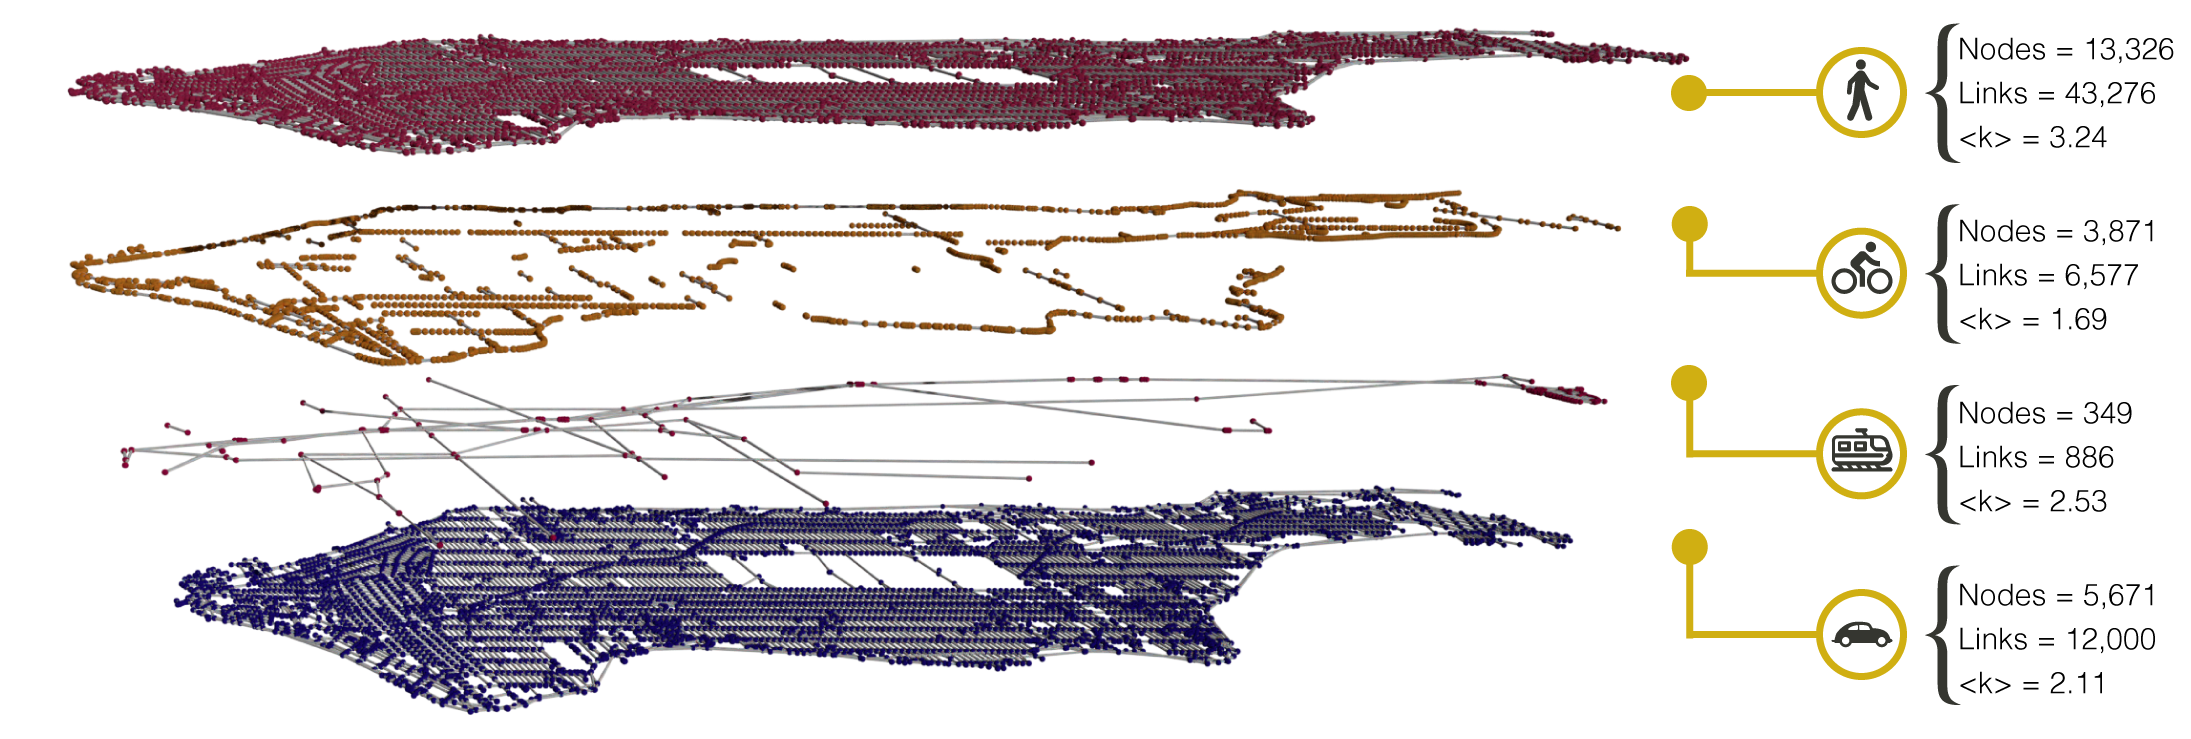
\includegraphics[width=\textwidth]{images/multiplex/Multilayer_NY_op2.png}
	\caption[Manhattan multiplex network]{\textbf{(Map plot left)} Multiplex network representation of Manhattan with the four analyzed layers of transport infrastructure (pedestrian paths, bicycle paths, rail lines, and streets), with data from OpenStreetMap. \textbf{(Right)} Network information for each layer, number of nodes, links and average degree $\langle k \rangle$.}
	\label{fig:ManhattanMultiplex}
\end{figure*}


\section{FINDINGS}
\begin{figure*}[t!]
	\centering
	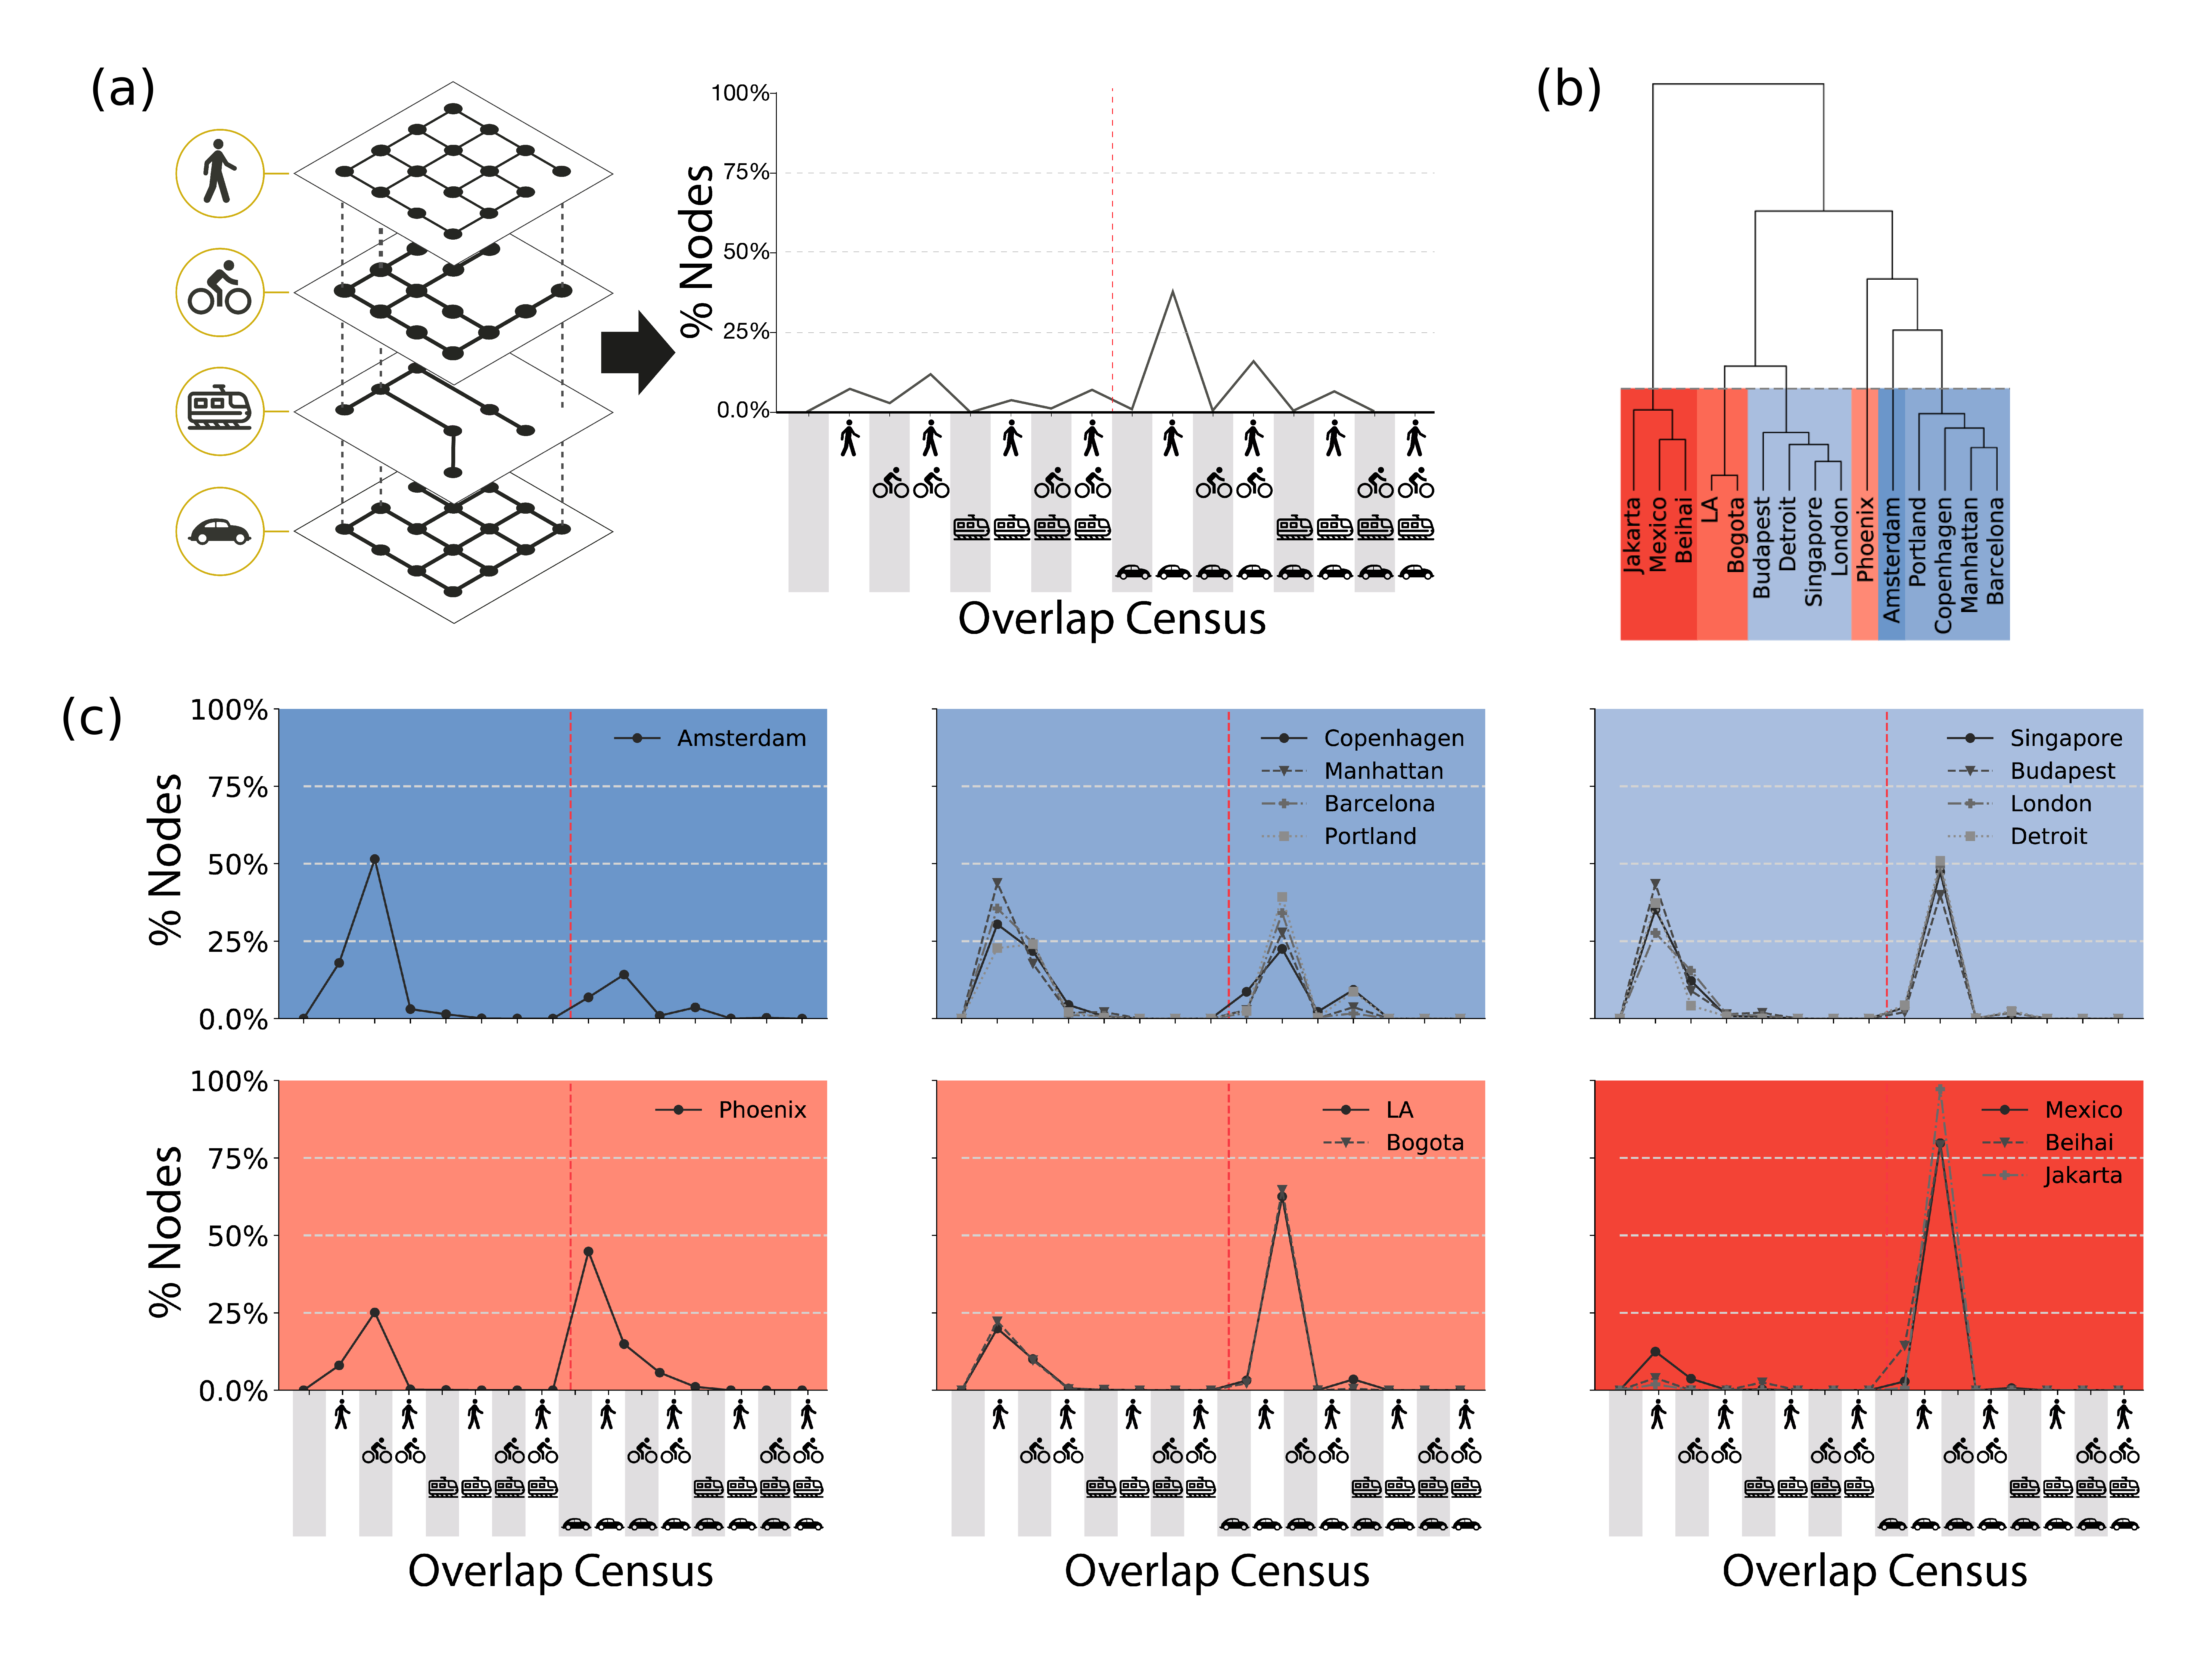
\includegraphics[width=\textwidth]{images/multiplex/Fig02.png}
	\caption[Overlap census configurations]{
		\textbf{(a)} Schematic of multiplex layers in a city (left) and its transformation to the overlap census (right). In the overlap census, the vertical red line gives a visual separation of the left from the right half where nodes become active in the street layer. High spikes in the right half indicate car-centricity.
		\textbf{(b)} Clusters of cities based on similarity of their overlap census. We find six different clusters using a k-means algorithm (coloured areas), which explain more than $90\%$ of the variance.
		\textbf{(c)} Overlap census for cities in each cluster. The first one corresponds to Amsterdam (the city with most active nodes in bicycle-only configurations). The Copenhagen-Manhattan-Barcelona-Portland city cluster has many active nodes in pedestrian-only and bicycle-only configurations, representing an active mobility city. The clusters of Los Angeles-Bogota and Mexico-Beihai-Jakarta are car-centric.}
	\label{fig:OverlapCensus}
\end{figure*}

Even in a multimodally ``optimal'' city there will be a high heterogeneity of node activities due to the different speeds and nature of transport modes, implying, for example, a much lower density of nodes necessary for a train network than for a bicycle network. Therefore, a good way to assess a city's overlap census is by comparing it with the overlap census of other cities. We find similarities between cities via a k-means algorithm fed with fifteen vectors (one per city), where each vector contains the percentages of nodes active in each possible configuration. The algorithm separates the 15 analyzed cities into six different clusters [Fig.~\ref{fig:OverlapCensus}(b)].

On the left half of the overlap census, we show the configurations in which nodes are not active in the street layer, while the right half contains car-related configurations [Fig.~\ref{fig:OverlapCensus}(c)] . These clusters of cities are useful to explain similarities in infrastructure planning in different transport development paths~\cite{Rodrigue2013Geography,Louf2014Typology}, with clusters of car-centric urbanization (like Mexico, Beihai, and Jakarta) opposed to clusters that show a more multimodal focus in their mobility infrastructure (like Copenhagen, Manhattan, Barcelona, and Portland). In the extreme cluster that contains only Amsterdam, close to $50\%$ of nodes are active in the bicycle layer, whereas in the Mexico-Beihai-Jakarta cluster more than $50\%$ of nodes are active in the street-pedestrian configuration. The concentration of nodes in just one configuration informs not only about the mobility character of the city, i.e. Amsterdam being a bicycle-friendly city, but unveils the importance of explicitly considering overlooked layers and their interconnections. For example, Singapore, Budapest, London, and Detroit have two main peaks indicating that most of their nodes are either active in the street-pedestrian or only in the pedestrian configuration. This is not the case in Los Angeles and Bogota, where the majority of nodes are active in the car-pedestrian combination, i.e. the pedestrians have to share most of the city with cars. Our multimodal fingerprint unravels how different transport modes are interlaced, helping identifying which layer (or set of layers) could be improved to promote multimodal, sustainable mobility.

To summarize, we propose the new ``overlap census'' method based on multiplex network theory allowing to rigorously identify and compare the multimodal potential of cities.
\pagestyle{fancy} %Multiplex fingerprint
\chapter{Data-driven strategies for optimal bicycle network growth}

Urban transportation networks, from sidewalks and bicycle paths to streets and rails, provide the backbone for movement and socioeconomic life in cities. To make urban transport sustainable, cities are increasingly investing to develop their bicycle networks. However, it is yet unclear how to extend them comprehensively and effectively given a limited budget. Here we investigate the structure of bicycle networks in cities around the world, and find that they consist of hundreds of disconnected patches, even in cycling-friendly cities like Copenhagen. To connect these patches, we develop and apply data-driven, algorithmic network growth strategies, showing that small but focused investments allow to significantly increase the connectedness and directness of urban bicycle networks. We introduce two greedy algorithms to add the most critical missing links in the bicycle network focusing on connectedness, and show that they outmatch both a random approach and a baseline minimum investment strategy. Our computational approach outlines novel pathways from car-centric towards sustainable cities by taking advantage of urban data available on a city-wide scale. It is a first step towards a quantitative consolidation of bicycle infrastructure development that can become valuable for urban planners and stakeholders.\footnote{A stand alone version of this chapter has been published in Royal Socity Open Science \cite{natera2020growth}}



\section{Prelude}
Most modern cities have followed a car-centric development in the 20th century \cite{Jacobs1961Death} and are today allocating a privileged amount of urban space to automobile traffic \cite{Gossling2016Space,Szell2018Crowdsourced}. From a network perspective, this space can be described as the street layer of a larger mathematical object, the multiplex transport network \cite{Morris2012Transport,Strano2015Features,Aleta2017Multilayer}. A city's multiplex transport network contains other network layers that have co-evolved with the street layer, such as the bicycle layer or the rail network layer, Fig.~\ref{fig:Multimodal}. Due to the car-centric development of most cities, street layers are the most developed layers and define or strongly limit other layers: For example, sidewalks are by definition footpaths along the side of a street and make up a substantial part of a city's pedestrian space \cite{Gossling2016Space}; similarly most bicycle paths are part of a street or are built along the side.

From an urban sustainability perspective, this situation is suboptimal because the unsustainable mode of automobile transportation dominates sustainable modes like cycling. Consequently, urban planning movements in a number of pioneering cities are increasingly experimenting with drastic policies, such as applying congestion charges (London) \cite{Eliasson2008Lessons} and repurposing or removing car parking (Amsterdam, Oslo) \cite{Littke2016parklets,bliss2019hcp,Nieuwenhuijsen2016Car}. These efforts agree in one common goal, together with the literature on cycling safety \cite{Reynolds2009impact,Teschke2012route,Pucher2016Safer,aldred2018cycling} and with cost-benefit analysis \cite{gossling2019social}: Protected bicycle lanes need to be extended considerably to create complete bicycle networks that provide a safe infrastructure for cycling citizens. Although scattered efforts in this direction have shown preliminary success, a quantitative framework for developing and assessing systematic strategies is missing \cite{Gossling2020Cities}.

Here we analyze the bicycle infrastructure network of 14 world cities, from leading bicycle-culture countries like Netherlands, to car-centric countries like Great Britain, the USA, or Colombia. We first uncover network fragmentation within the bicycle dedicated infrastructure. Then, to improve a city's vital dedicated bicycle infrastructure \cite{Dill2013Bicycle,Schoner2014Missing,Hull2014Infrastructure,Buehler2016Bikable}, we develop algorithms for connecting disconnected graphs based on concrete quality metrics from bicycle network planning \cite{Twaddell2018Multimodal} and apply them to the empirical bicycle networks via network growth simulations. We find that localized investment into targeted missing links can rapidly consolidate fragmented bicycle networks, allowing to significantly increase their connectedness and directness, with potentially crucial implications for sustainable transport policy planning.

\begin{figure}[th!]
  \centering
  \includegraphics[width=\textwidth]{images/datadriven/Fig01.png}
  \caption[Multimodal configuration]{\textbf{(Map plots, left)} Networks representing various layers of transport infrastructure (pedestrian paths, bicycle paths, rail lines, and streets) for Copenhagen and London, with data from OpenStreetMap. \textbf{(Right)} Connected component size distribution $P(N_{cc})$ as a function of the ranking of the component for all considered network layers and cities. All layers are well connected except the bicycle layer: Copenhagen has 321 bicycle network components despite being known as a bicycle-friendly city, while London's bicycle layer is much more fragmented, featuring over 3000 disconnected components. Copenhagen's largest connected bicycle component (leftmost data point) spans 50\% of the network, but London's only less than 5\%.}
  \label{fig:Multimodal}
\end{figure}

\section{Data acquisition and network construction}
We acquired street and bicycle infrastructure networks from multiple cities around the world using OSMnx \cite{Boeing2017OSMNX}, a Python library to download and construct networks from OpenStreetMap (OSM). OSMnx simplifies the OpenStreetMap's raw data to retain only nodes at the intersections and dead ends of streets, and the spatial geometry of the edges, generating a length-weighted nonplanar directed graph \cite{Boeing2020Planarity}. These data sets are of high quality \cite{Haklay2010OpenStreetMap,Girres2010Quality} in terms of correspondence with municipal open data \cite{Ferster2019Bicycle} and completeness: More than $80\%$ of the world is covered by OSM \cite{Barbosa-Filho2017Models}. In particular, OSM's bicycle layer has better coverage than proprietary alternatives like Google Maps \cite{Hochmair2012}. We collect data from a diverse set of cities to capture different development states of bicycle infrastructure networks; from consolidated networks like Amsterdam and Copenhagen, less developed ones like Manhattan and Mexico City, to rapidly developing cities like Jakarta and Singapore. The various analyzed urban areas and their properties (number of nodes $N$, number of connected components $CC$, and population) are reported in Table~\ref{tab:DataDrivenCities}. Code to replicate our results is available as Jupyter Notebooks (\url{https://github.com/nateraluis/bicycle-network-growth}) and data can be downloaded from Harvard Dataverse \cite{natera2019data}.

\begin{table*}[th!]
  \centering
  \begin{adjustbox}{width=0.9\textwidth,keepaspectratio}
    \begin{tabular}{llllllllllllll}
      \toprule
      {}         & \multicolumn{3}{l}{walk} & \multicolumn{3}{l}{bike} & \multicolumn{3}{l}{rail} & \multicolumn{3}{l}{drive} & Population                                                                                                             \\
      {}         & $N$                      & $CC$                     & $\ell(km)$               & $N$                       & $CC$       & $\ell(km)$ & $N$     & $CC$ & $\ell(km)$ & $N$       & $CC$ & \multicolumn{2}{l}{$\ell(km)$}              \\
      \midrule
      Amsterdam  & 23,321.0                 & 1.0                      & 2,075.67                 & 34,529.0                  & 355.0      & 972.08     & 1,096.0 & 8.0  & 288.72     & 15,125.0  & 1.0  & 2,010.49                       & 872,680    \\
      Barcelona  & 20,203.0                 & 1.0                      & 2,122.6                  & 7,553.0                   & 122.0      & 229.19     & 263.0   & 29.0 & 105.98     & 10,393.0  & 1.0  & 1,551.44                       & 1,600,000  \\
      Bogota     & 81,814.0                 & 1.0                      & 8,686.51                 & 9,760.0                   & 171.0      & 367.33     & 166.0   & 12.0 & 20.2       & 62,017.0  & 1.0  & 7,383.69                       & 7,412,566  \\
      Budapest   & 73,172.0                 & 1.0                      & 7,746.12                 & 10,494.0                  & 257.0      & 336.13     & 1,588.0 & 20.0 & 522.06     & 37,012.0  & 1.0  & 5,332.97                       & 1,752,286  \\
      Copenhagen & 30,746.0                 & 1.0                      & 2,286.66                 & 13,980.0                  & 321.0      & 417.01     & 276.0   & 3.0  & 123.56     & 15,822.0  & 1.0  & 1,547.3                        & 2,557,737  \\
      Detroit    & 47,828.0                 & 1.0                      & 6,769.46                 & 3,663.0                   & 53.0       & 141.06     & 20.0    & 3.0  & 11.54      & 28,462.0  & 1.0  & 5,624.49                       & 672,662    \\
      Jakarta    & 140,042.0                & 1.0                      & 13,947.96                & 248.0                     & 19.0       & 8.44       & 60.0    & 8.0  & 81.24      & 138,388.0 & 1.0  & 14,194.2                       & 10,075,310 \\
      LA         & 89,543.0                 & 1.0                      & 14,329.92                & 14,577.0                  & 230.0      & 653.16     & 173.0   & 9.0  & 90.82      & 71,091.0  & 1.0  & 13,324.46                      & 3,792,621  \\
      London     & 270,659.0                & 1.0                      & 23,846.62                & 62,398.0                  & 3,023.0    & 1,281.71   & 2,988.0 & 38.0 & 1,045.39   & 179,782.0 & 1.0  & 18,154.52                      & 8,908,081  \\
      Manhattan  & 13,326.0                 & 1.0                      & 1,320.78                 & 3,871.0                   & 105.0      & 111.42     & 349.0   & 5.0  & 197.51     & 5,671.0   & 1.0  & 1,022.13                       & 1,628,701  \\
      Mexico     & 108,033.0                & 1.0                      & 14,547.18                & 5,218.0                   & 52.0       & 332.37     & 371.0   & 18.0 & 253.48     & 95,375.0  & 1.0  & 13,732.39                      & 8,918,653  \\
      Phoenix    & 111,363.0                & 1.0                      & 14,314.0                 & 35,631.0                  & 141.0      & 1,221.18   & 105.0   & 4.0  & 71.64      & 73,688.0  & 1.0  & 11,841.49                      & 1,445,632  \\
      Portland   & 50,878.0                 & 1.0                      & 5,324.78                 & 24,252.0                  & 198.0      & 596.36     & 230.0   & 2.0  & 132.36     & 35,025.0  & 1.0  & 4,583.47                       & 583,776    \\
      Singapore  & 82,808.0                 & 1.0                      & 8,633.13                 & 12,981.0                  & 104.0      & 339.39     & 683.0   & 14.0 & 428.66     & 50,403.0  & 1.0  & 6,635.37                       & 5,638,700  \\
      \bottomrule
    \end{tabular}
  \end{adjustbox}
  \caption[Measures for analyzed cities]{Measures for the administrative area of analyzed cities. The number of connected components ($CC$) and nodes ($N$) for each layer in all cities of our dataset are highly diverse due to the varying developmental levels and focus of transport.
    \label{tab:DataDrivenCities}}
\end{table*}

We characterize each city street and bicycle infrastructure as a primal network, \cite{Porta2006Primal} in which nodes are intersections, while links represent bicycle paths, and designated bicycle infrastructure. This recent approach has been useful to demonstrate how cities grow \cite{Strano2012Evolution,Barthelemy2013Evolution}, how efficient \cite{Gallotti2014Efficiency} and dense they are, and to capture the tendency of travel routes to gravitate towards city centers \cite{Lee2017Morphology}. This network is described by an adjacency matrix $A=\{a_{ij}^{[\alpha]}\}$ where $a_{ij}=1$ if there is a link between nodes $i$ and $j$ and 0 otherwise.

\section{Defining bicycle network growth strategies and quality metrics}
Across all cities considered, we find that almost all network layers are made up of one giant component, except for the bicycle layer which is always fragmented into many disconnected components (see Table~\ref{tab:DataDrivenCities}). This discovery is remarkable given that the fragmentation occurs also in bicycle-friendly cities like Copenhagen (Fig.~\ref{fig:Multimodal}), showing that cycling infrastructure can be suboptimal even in the leading cycling cities on the planet. To quantify such an underdevelopment in the sustainable mobility infrastructure of cycling, we focus on the single layer of bicycle networks and on two well-established metrics in bicycle infrastructure quality assessment \cite{Krizek2005Discontinuities,movement2013Cycling,Dobrovolny2014Pedestrian,Twaddell2018Multimodal,Beck2019Space}: \textit{connectedness} and \textit{directness}. Connectedness indicates ``the ease with which people can travel across the transportation system'' \cite{Twaddell2018Multimodal}, and it is related to answering the question ``can I go where I want to, safely?''. Directness addresses the question ``how far out of their way do users have to travel to find a facility they can or want to use?'', and can be measured by how easy it is to go from one point to another in a city using bicycle infrastructure versus other mobility options, like car travel.

As our main approach, we choose to measure connectedness and directness over the designated bicycle infrastructure only, without considering travel on streets. Although it is possible to cycle on streets, growing evidence from bicycle infrastructure and safety research is unveiling serious safety issues for cycling when mixed with vehicular traffic \cite{Reynolds2009impact,Teschke2012route,Pucher2016Safer}. However, we also tested our algorithms on a combination of bicycle infrastructure plus streets for which the maximum speed is $30\,\mathrm{km/h}$, following common best-practice reasoning that low speed limits can make streets safe for cycling \cite{global2016global}. The results of these additional simulations are available in the Supplementary Information; they do not differ significantly from the case of designated bicycle infrastructure presented below, as the developed algorithms follow the same rules to connect the multiple components in both cases of segregated bicycle infrastructure only and of included bikeable streets.

To quantify connectedness, we first measure the number of disconnected components of each city's bicycle network. It is no surprise that car-centric cities have a highly fragmented bicycle infrastructure: for example, London has more than 3,000 disconnected bicycle infrastructure segments. However, even bicycle-friendly cities like Copenhagen have over 300 disconnected bicycle path components -- see the connected component size distribution $P( N_{cc} )$ in Fig.~\ref{fig:Multimodal}. This infrastructure fragmentation in the bicycle layer poses a challenge for a city's multimodal mobility options \cite{natera2020multimodal} and for the safety of its cycling citizens \cite{Dill2009infrastructure,Chataway2014Safety}.

There are various approaches in developing automated strategies for bicycle infrastructure planning. Hyodo et al.~\cite{Hyodo2000Modeling} have proposed a bicycle route choice model to plan bicycle lanes taking into account facility characteristics. Other studies have used input data from bicycle share systems \cite{Bao2017Planning} or origin destination matrices \cite{Mauttone2017Design} to plan bicycle lanes. More recently, taxi trips have been used to identify susceptible clusters for bicycle infrastructure \cite{Akbarzadeh2018Design}. Here we attempt an alternative approach: Since hundreds of bicycle network components already exist in most cities, we aim at consolidating the existing infrastructure by making strategic connections between components rather than starting from scratch.


\begin{algorithm}[h!]
  \begin{algorithmic}[1]
    \Procedure{\textit{L2S}}{}
    \State $\textit{G} \gets \text{ bicycle network graph}$
    \State $\textit{wcc} \gets \text{ components of network G}$
    \For {i in length(wcc)-1}
    \State  \text{sort \textit{wcc} by components size}
    \State $\textit{cc} \gets \text{ two biggest components from \textit{wcc}}$
    \State $\textit{i\_j} \gets \text{ closest nodes between } cc_0 \text{ and } cc_1$
    \State $\text{connect } cc_0 \text{ and } cc_1 \text{ in } i\_j$
    \EndFor
    \EndProcedure
  \end{algorithmic}
  \caption{Largest-to-Second. \textcolor{blue}{The algorithm takes the bicycle network \textit{G} and a list of its weakly connected components \textit{wcc}, then it iterates over the weakly connected components, sorts them by their size (number of nodes inside each component), locates the closest pairs of nodes between the first and the second components. The process is repeated until all the components have been connected.}}\label{al:L2S}
\end{algorithm}

\begin{algorithm}[h!]
  \caption{Largest-to-Closest. \textcolor{blue}{The algorithm takes the bicycle network \textit{G} and a list of its weakly connected components \textit{wcc}, then it iterates over the weakly connected components, sorts them by their size (number of nodes inside each component), locates the largest connected component and the closest of the remaining components, the components are connected. The process is repeated until all the components have been connected.}}\label{al:L2C}
  \begin{algorithmic}[1]
    \Procedure{\textit{L2C}}{}
    \State $\textit{G} \gets \text{ bicycle network graph}$
    \State $\textit{wcc} \gets \text{ components of network G}$
    \For {i in length(wcc)-1}
    \State  \text{sort \textit{wcc} by components size}
    \State $cc_0 \gets \text{ biggest component from \textit{wcc}}$
    \State $cc_n \gets \text{ clossest component to } cc_0$
    \State $\textit{i\_j} \gets \text{ closest nodes between } cc_0 \text{ and } cc_n$
    \State $\text{connect } cc_0 \text{ and } cc_n \text{ in } i\_j$
    \EndFor
    \EndProcedure
  \end{algorithmic}
\end{algorithm}

Our approach takes into account the currently available bicycle infrastructure and uses an algorithmic process to improve the network by finding the most important missing links step by step. This way we focus on optimizing the connectedness metric, growing the bicycle infrastructure by making it more connected, merging parts into fewer and fewer components. We develop two iterative greedy algorithms that we check against a random and a minimum investment approach. The first algorithm, \emph{Largest-to-Second} (L2S), identifies in each step the largest connected component in the bicycle infrastructure network and connects it to the second largest (see algorithm~\ref{al:L2S} for details). The second algorithm, \emph{Largest-to-Closest} (L2C), also identifies the largest connected component, but connects it to the closest of the remaining bicycle infrastructure components (see algorithm~\ref{al:L2C} for details). In both algorithms, components are connected through a direct link between their two closest nodes. We use this technique as an approximation to the underlying street-shortest path -- since the most relevant shortest 100 connections typically range from $14$ to $500$ meters, roughly the length of two blocks, this approximation is reasonable. The algorithms repeat this process until there are no more disconnected components in the network.

To have a random baseline, we compare our algorithms with a \emph{Random-to-Closest} (R2C) component approach. In each step of this baseline approach, one component is picked at random and connected with the closest remaining one (see algorithm~\ref{al:R2C} for details). This baseline allows us to model a scenario where infrastructure is developed following a systematic but random linking approach -- in urban development this corresponds to uncoordinated local planning that randomly connects close pieces of bicycle infrastructure. We also implement a second baseline, the extreme case of \emph{Closest-Components} (CC), which prioritizes connecting the closest two components disregarding their size (see algorithm~\ref{al:CC} for details). This CC approach is equivalent to an ``invest as little as possible'' development strategy -- it builds up a minimum-spanning-tree-like structure  following a modified Kruskal's algorithm \cite{Kruskal1956Spanning}. All four algorithms connect components optimizing a well-defined criterion, finding the critical missing links in the network, and adding one new link per iteration. See Fig.~\ref{fig:algorithms} for a schematic of the four algorithms.


\begin{algorithm}[h!]
  \caption{Random-to-Closest. \textcolor{blue}{The algorithm takes the bicycle network \textit{G} and a list of its weakly connected components \textit{wcc}, then it iterates over the weakly connected components, randomly picks a component and connects it to the closest of the remaining components. The process is repeated until all the components have been connected.}}\label{al:R2C}
  \begin{algorithmic}[1]
    \Procedure{\textit{R2C}}{}
    \State $\textit{G} \gets \text{ bicycle network graph}$
    \State $\textit{wcc} \gets \text{ components of network G}$
    \For {i in length(wcc)-1}
    \State $cc_{ran} \gets \text{ random component from \textit{wcc}}$
    \State $cc_n \gets \text{ clossest component to } cc_{ran}$
    \State $\textit{i\_j} \gets \text{ closest nodes between } cc_{ran} \text{ and } cc_n$
    \State $\text{connect } cc_{ran} \text{ and } cc_n \text{ in } i\_j$
    \EndFor
    \EndProcedure
  \end{algorithmic}
\end{algorithm}

\begin{algorithm}[h!]
  \caption{Closest-Components. \textcolor{blue}{The algorithm takes the bicycle network \textit{G} and a list of its weakly connected components \textit{wcc}, then it iterates over the weakly connected components, calculate the distance between available components and connect the two closests ones. The process is repeated until all the components have been connected.}}\label{al:CC}
  \begin{algorithmic}[1]
    \Procedure{\textit{CC}}{}
    \State $\textit{G} \gets \text{ bicycle network graph}$
    \State $\textit{wcc} \gets \text{ components of network G}$
    \For {i in length(wcc)-1}
    \State $\Delta_{min} \gets \text{ clossest components in \textit{wcc}}$
    \State $cc_{0} \gets \text{ first component for }\Delta_{min}$
    \State $cc_{1} \gets \text{ second component for } \Delta_{min}$
    \State $\textit{i\_j} \gets \text{ closest nodes between } cc_{0} \text{ and } cc_{1}$
    \State $\text{connect } cc_{0} \text{ and } cc_{1} \text{ in } i\_j$
    \EndFor
    \EndProcedure
  \end{algorithmic}
\end{algorithm}

We apply the algorithms to the bicycle infrastrucutre inside the political demarcation of the cities, however it is possible to extend the methods and include bicycle highways and cross-city trails, since they use as input a set of spatial network components to connect. We opt to not include cross-city links, since they are a special case only available in a few regions and where adequate intra-urban bicycle infrastructure has already been established \cite{Hildebrandt2013BicycleHighways,Taciuk2018Bicycle}.

To test how much cities improve their bicycle layers using these four algorithms, we define two metrics on the bicycle layer that operationalize the notion of connectedness: i) $n_{LCC} = \frac{N_{LCC}}{N} $, the fraction of nodes from the bicycle infrastructure inside the largest connected component ($N_{LCC}$) compared to the total number of nodes from the same type of infrastructure ($N$), and ii) $\ell_{LCC} = \frac{L_{LCC}}{L} $, the fraction of link kilometers inside the bicycle infrastructure largest connected component ($L_{LCC}$) compared to the total number of link kilometers in the bicycle network ($L$). Both metrics take values between 0 and 1, where 1 means that there is only one connected component. An intermediate value, for example 0.2, means that the largest connected component contains 20\% of all bicycle intersections or path kilometers. Executing our algorithms step by step these metrics can only grow, approaching 1 when the process is complete and they terminate. What distinguishes the algorithms is \emph{how fast} these values grow.

\begin{figure}[t!]
  \centering
  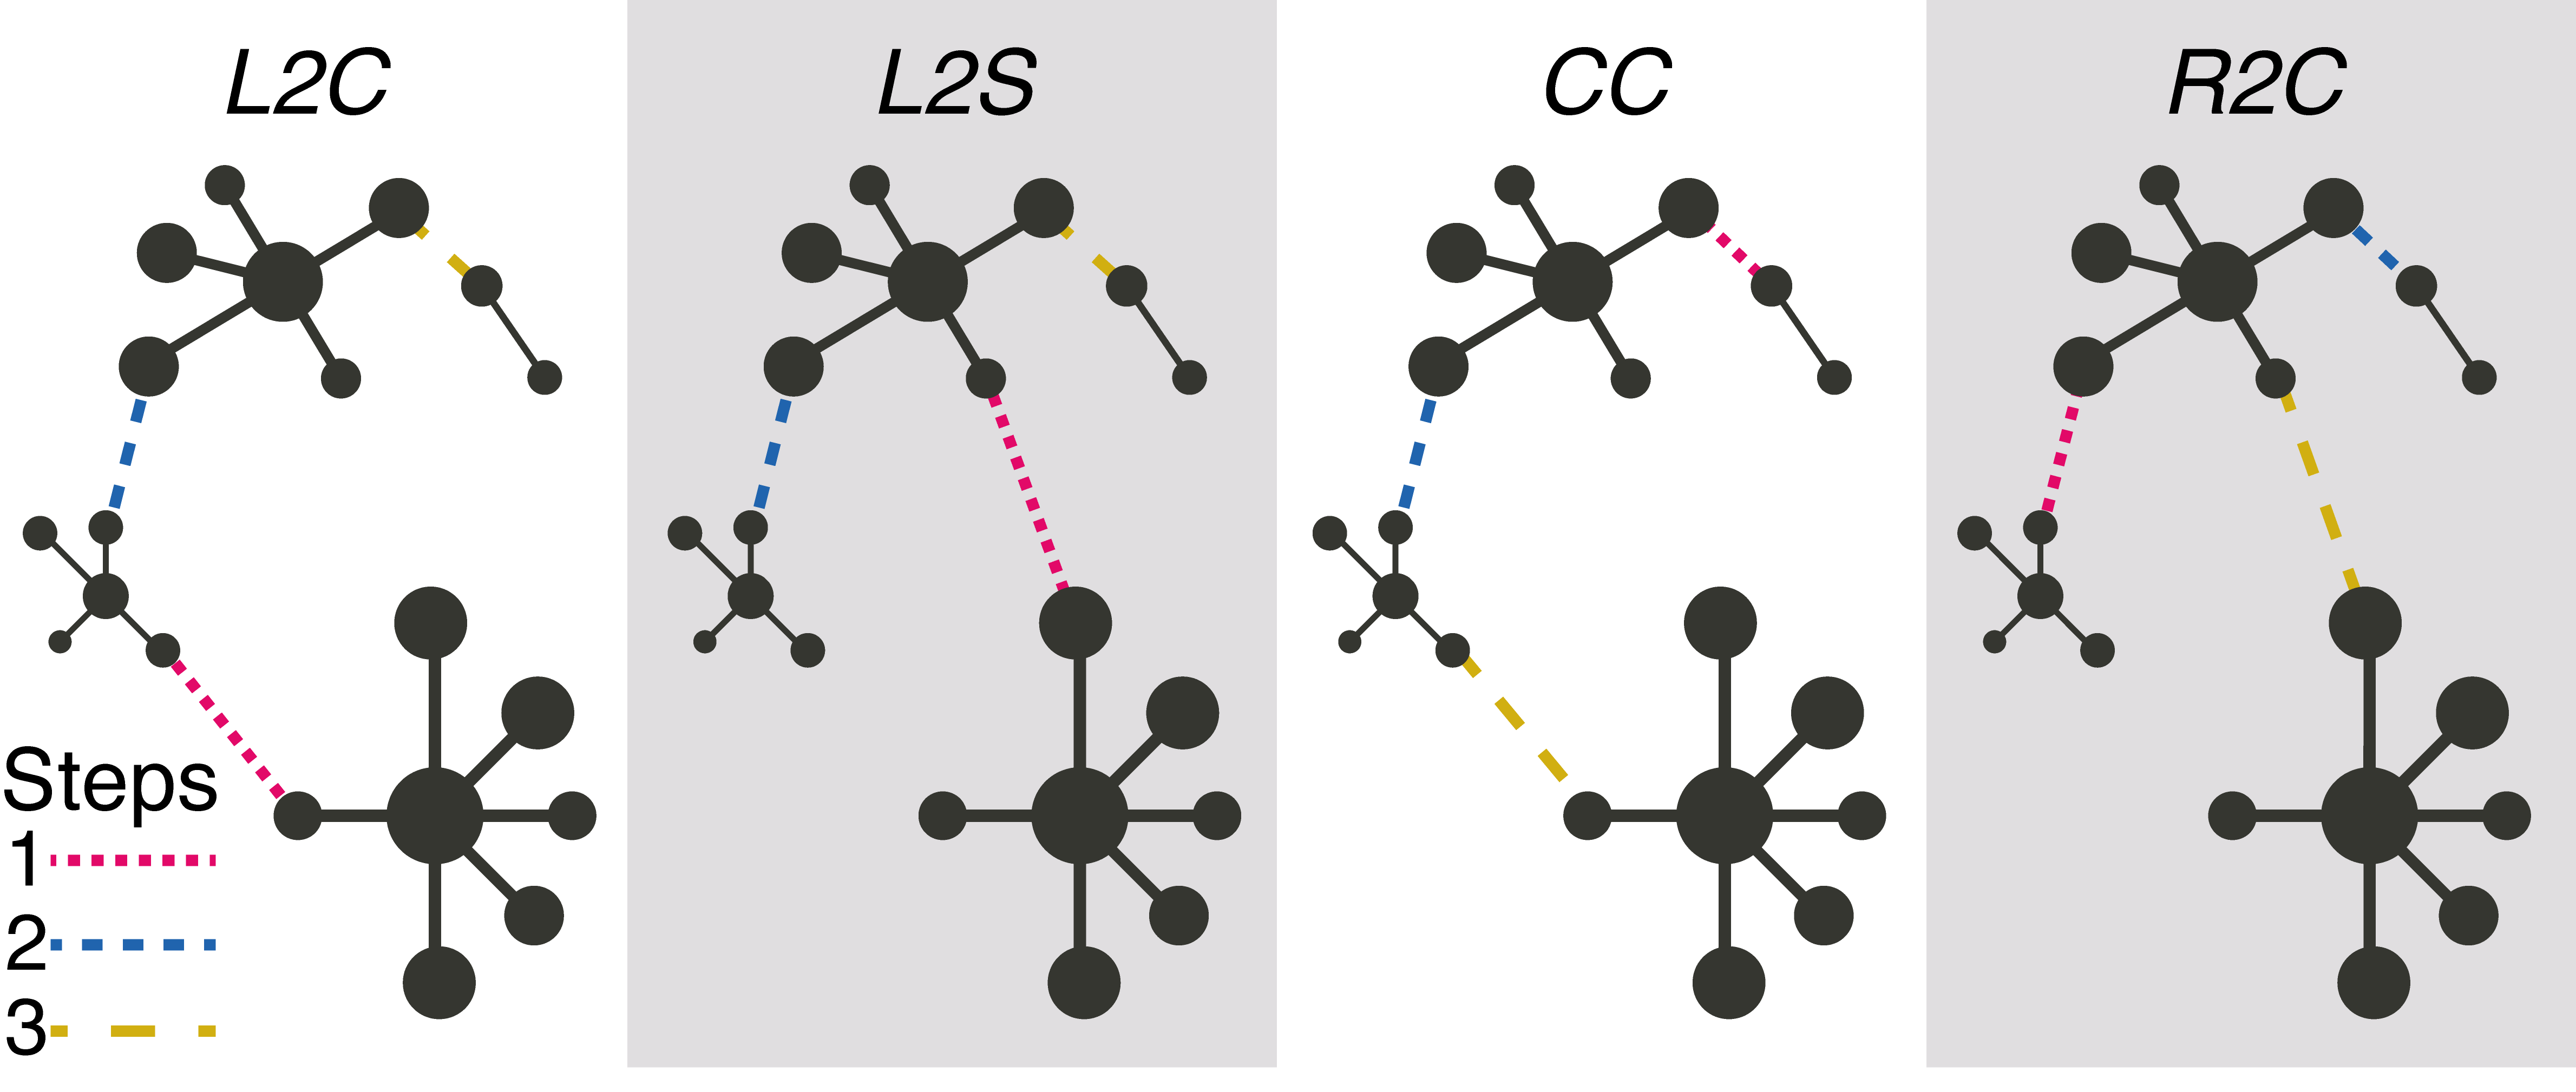
\includegraphics[width=\textwidth]{images/datadriven/algorithms.png}
  \caption[Algorithms schematic representation]{Schematic representation of algorithms to improve bicycle network infrastructure: Largest-to-Closest (L2C) finds the largest component and connects it with the closest one; Largest-to-Second (L2S) connects the largest component with the second largest; Closest-Connected (CC) connects the two closest components; and Random-to-Closest (R2C) picks a random component and connects it to the closest.}
  \label{fig:algorithms}
\end{figure}

We quantify directness through the metric: iii) bicycle-car directness $\Delta$, which answers the question ``how direct are the average routes of bicycles compared to cars?'' via the ratio between average distance by car and average distance by bicycle. For example, if the shortest car-route from west to east Manhattan is 4\,km and the shortest route on the bicycle network between these two points is 5\,km, the bicycle-car directness is $4/5 = 0.8$. Note that if the bicycle network is a subset of the street network, then $\Delta$ cannot be larger than $1$. Formally we write $\Delta=\frac{\langle\delta_{ij}^b\rangle_{ij}}{\langle\delta_{ij}^s\rangle_{ij}}$, where $\langle\delta_{ij}^{s}\rangle_{ij}$ is the average car-route distance, and $\langle\delta_{ij}^{b}\rangle_{ij}$ is the average length of the shortest bike-route between $i$ and $j$. In each iteration of any of our algorithms, we implement this measure by randomly selecting one thousand pairs of origin-destinations nodes and then averaging the corresponding street/bicycle distance. To avoid undefined values due to disconnected components in the bicycle layer, we add the following condition: If a node from the pair \textit{i} and \textit{j} is in a different component, we assign the value $\delta_{ij}^{b} = 0$. This condition also ensures consistency of growing directness values while the algorithm merges more and more nodes into the same component.

Finally, in order to measure the cumulative efficiency of our algorithms, we define the metric: iv) $G_{LCC}$ as the relative gain of bicycle path kilometers in the largest connected component. For example, $G_{LCC}=1.5$ means that the algorithm has increased the largest connected component's original size by 150\%. Formally, $G_{LCC}=\frac{L_{LCC}-L_{LCC_0}}{L_{LCC_0}}$, where $L_{LCC_0}$ is the sum of kilometers in the largest connected component before the algorithm runs. As with all other metrics, $G_{LCC}$ is monotonically increasing with the growth algorithm, and reaches $\frac{1-\ell_{LCC_0}}{\ell_{LCC_0}}$ at the end of the dynamics.

\section{Growing bicycle networks shows stark improvements with small investments}

\begin{figure}[htbp]
  \centering
  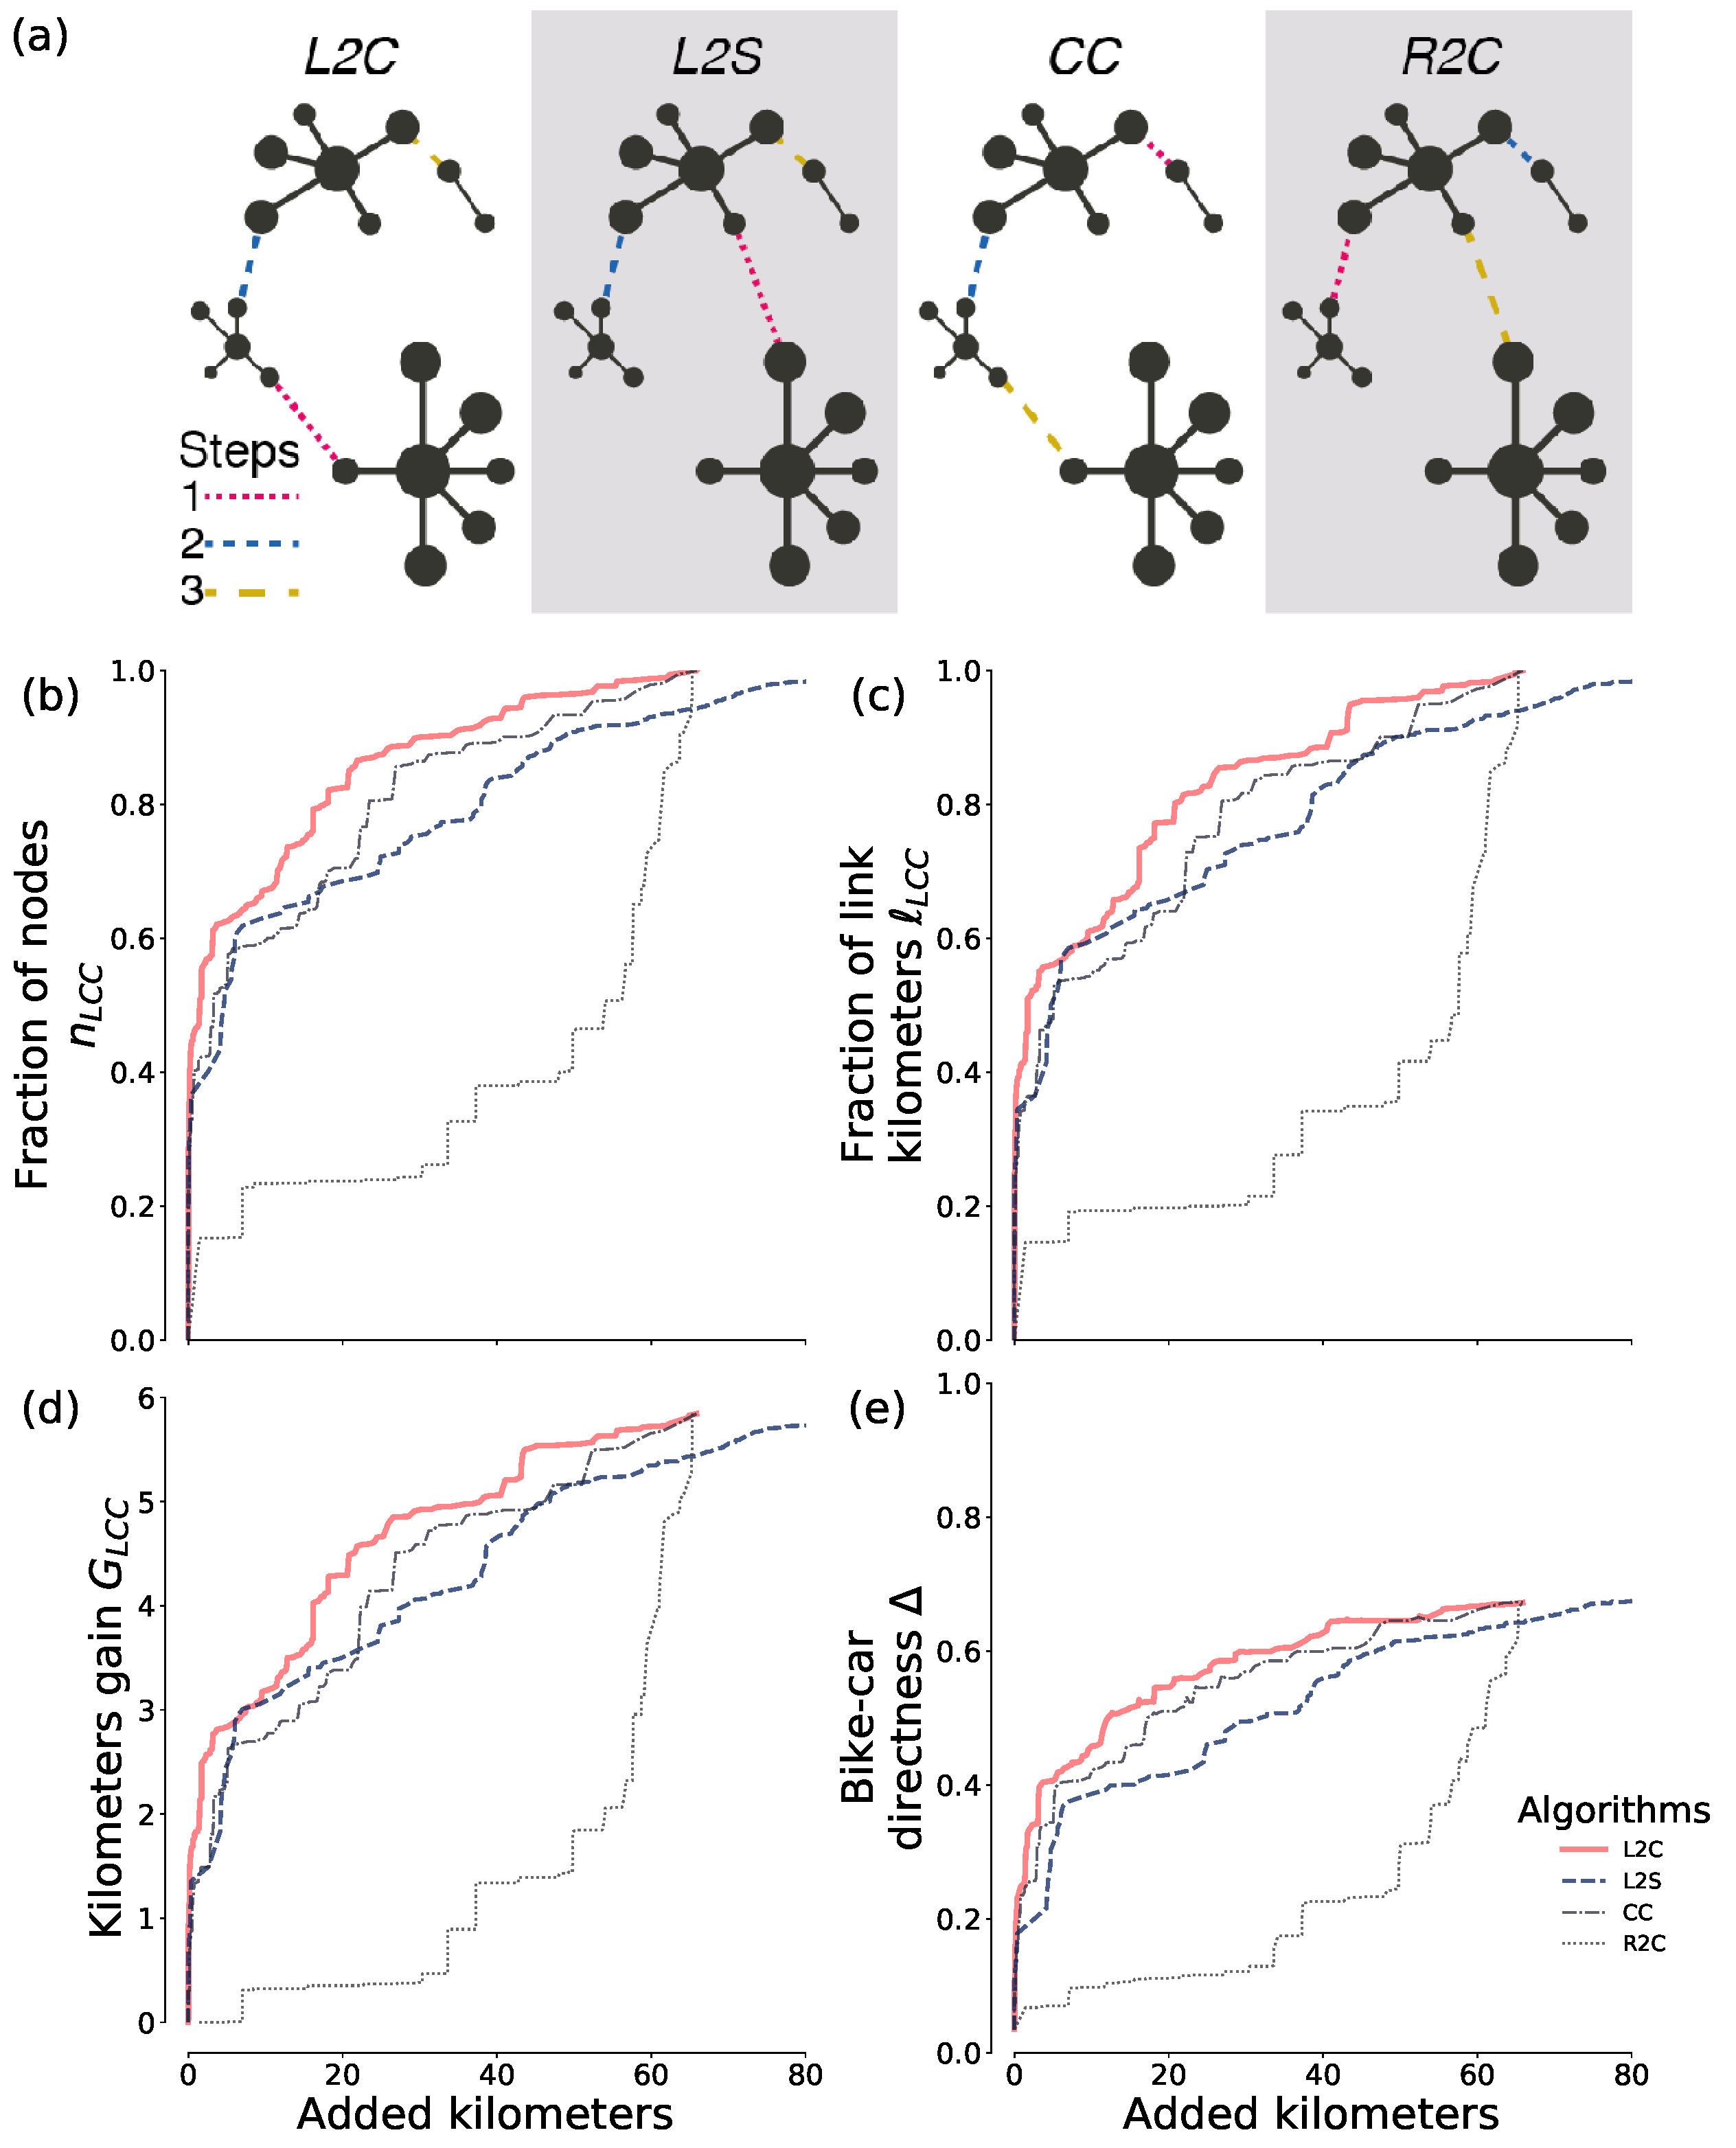
\includegraphics[width=\textwidth]{images/datadriven/Fig03.pdf}
  \caption[Algorithmic improvement in Budapest]{\textbf{(b)} Normalized increase in nodes inside the largest connected component ($n_{LCC}$). \textbf{(c)} Normalized increase in kilometers inside the largest connected component ($\ell_{LCC}$). \textbf{(d)} Kilometers gain ($G_{LCC}$). \textbf{(e)} Bicycle-car directness ($\Delta$). Measures in (b-e) are plotted as a function of the sum of added links in kilometers, for the case of Budapest (for all cities see Fig.~\ref{fig:Nodes})}
  \label{fig:ImprovementBP}
\end{figure}

We demonstrate in Fig.~\ref{fig:ImprovementBP} the power of the various growth strategies by showing the initial state of the bicycle layer for the case of Budapest and its state after 85 iterations of the \emph{Largest-to-Closest} algorithm: At this point the network has almost quadrupled the size of its largest connected component (from 82\,km to 313\,km), with a negligible investment of just less than 5\,km (corresponding to $1.4\%$ of the previously existing bicycle infrastructure) in new connecting bicycle paths. In terms of connectedness, it goes from $15\%$ to $56\%$ connected. This rapid increase shows that the city can easily improve its bicycle infrastructure with small investments. For some extreme cases, like Bogota, with the same 5\,km investment (an increase of $1.3\%$ to the previously existing infrastructure) the bicycle-car directness increases from $6\%$ to almost $48\%$ and connectedness from $34\%$ to $89\%$. Similar encouraging results hold for other cities, and for all the cities when taking into account the combination of bicycle infrastrucutre and safely bikeable streets ($\leq 30\,\mathrm{km/h}$)(see SI).

The fraction of nodes inside the largest connected component increases rapidly with newly added links for all considered algorithms except \emph{Random-to-Closest}, Fig.~\ref{fig:ImprovementBP}(b). The \emph{Largest-to-Closest} algorithm performs better than the others, even more than \emph{Closest-Components} which prioritizes minimum investments in the network. Since we are considering bicycle infrastructure, a better practical measure than the number of intersections is the number of kilometers that can be cycled using only designated paths. Figure~\ref{fig:ImprovementBP}(c) shows how this measure improves in a similarly explosive way: with an investment of only 20\,km ($5.9\%$ of the existing infrastructure), the largest connected component will contain $~80\%$ of the original bicycle infrastructure. Results for the kilometer gain $G_{LCC}$ are shown in Fig.~\ref{fig:ImprovementBP}(d). Three of the four algorithms rapidly gain new kilometers, but as the invested new kilometers grow, each algorithm follows a different gain rate. Also for this metric, \textit{Largest-to-Closest} is the algorithm with the best performance.

We also measure the bicycle-car directness ratio, Fig.~\ref{fig:ImprovementBP}(e). The bicycle-car directness $\Delta$ improves as the algorithms consolidate the network. These improvements are, however, indirectly driven by the improvement of connectedness, which boosts the accessibility of bicycles to different areas of the city. The flattening of the curves at a value considerably smaller than 1 (around 0.65) shows that cars will always outperform bicycles in terms of directness, having on average at least 33\% shorter paths in the city. This suboptimal flattening is a natural consequence of the algorithms optimizing for connectedness only, not adding ``redundant'' connections. Nevertheless, the measure shows that, similar to connectedness, with a relatively negligible investment of bicycle path kilometers into the system, the bicycle network's directness improves drastically, even in the greediest case where the shortest possible missing link is added in every iteration. This result holds for all analyzed cities (see SI). The large differences between the baseline \emph{Random-to-Closest} and our two algorithms (\emph{Largest-to-Second} and \emph{Largest-to-Closest}) show the importance of following an approach that consolidates and grows the largest connected component.

\section{Different cities have different optimal investment strategies}

\begin{figure}[htbp!]
  \centering
  \includegraphics[width=\textwidth]{images/datadriven/Fig04.pdf}
  \caption[Cities bicycle connectivity improvement]{Cities improvement and ranking using the \emph{Largest-to-Closest} algorithm. We report the improvement and ranking on the fraction of total kilometers of bicycle infrastructure in the largest connected component ($\ell_{LCC}$) and in the bicycle-car directness ($\Delta$). Dotted lines show thresholds of $25\%$, $50\%$, and $75\%$. Plots (a-b) show investment strategies of 5\,km and 35\,km, respectively, the Manhattan, London, and Budapest plots show the suggested new links (red) after adding 5\,km and 35\,km, the newly created largest connected component (black), and the remaining separated components (grey).}
  \label{fig:Improvement}
\end{figure}

Differences arise in the state of the bicycle layer and its improvement after applying a growth algorithm. To see this effect, we rank how cities improve using the \textit{Largest-to-Closest} algorithm in two different investment scenarios: investing either i) 5\,km, or ii) 30\,km. Figure~\ref{fig:Improvement}(a) shows how cities improve when investing 5\,km of bicycle infrastructure. We see that some cities get above $75\%$ of their existing infrastructure connected, meaning that their bicycle layer only needs a small extension. On the other hand, cities like London, Los Angeles, and Jakarta need a larger investment to improve. Concerning bicycle-car directness, cities reach lower values due to the focus of the algorithms on completeness. In the worst performing cities like Los Angeles, a covered length close to $50\%$ can be reached easily, while the bicycle-car directness ratio stays below $20\%$, showing that it is much harder to gain an acceptable bicycle infrastructure in cities where cars are overprioritized. The 35\,km investment strategy shows that most cities can get at least $75\%$ of their bicycle infrastructure connected, Fig.~\ref{fig:Improvement}(b). The worst performing outlier is London, due to its bicycle layer containing more than 3000 connected components scattered around $1600$ km$^2$ (see Table \ref{tab:DataDrivenCities}). In terms of bicycle-car directness London also performs badly, while Amsterdam is the best performing one.

The four proposed metrics capture the impact of newly created connections on the various components of the bicycle network. By linking previously disconnected neighbourhoods with a sustainable mode of transport, our approach focuses on consolidating bicycle infrastructure networks, thus making cities more cohesive and green. It does not, however, focus on growing the bicycle network into large areas of the city not currently served. To test to which extent such connectedness-based algorithms bring an indirect benefit for coverage, we measured the proportion of the city that is covered and reachable by bicycle with an epsilon of 500 meters around the bicycle infrastructure of the largest connected component, and calculated the percentage of nodes in the street layer that are covered by the bikeable area. The results of this measurement show a wide range of effects: Cities with an already high coverage above 80\% (Amsterdam, Copenhagen) reach near instantly 100\%, cities with an intermediate coverage (Manhattan, Bogota, Budapest) follow a more linear progression per added kilometer, while underdeveloped or sprawling cities (LA, London, Jakarta) show negligible growth (Fig.~\ref{fig:Coverage}).

While our present goal (consolidation of the bike network) is intended to show the potential of our approach, an extension towards the exploration of new city areas will increase further the real-world applicability of our results. We consider this extension an interesting line of future research in the challenge of developing optimal data-driven strategies of transport network growth, potentially informed by theoretical frameworks such as optimal percolation~\cite{achlioptas2009explosive,morone2015influence}. Besides, the use of other network metrics, such as network efficiency~\cite{latora2000efficient}, might unveil new dimensions characterising the impact of the proposed algorithms on the development of the bicycle infrastructure.


\section{Discussion}
Our starting point showed that a common characteristic of cities is the fragmentation of their bicycle networks. We have proposed the use of data-driven algorithms to consolidate bicycle network components into connected networks to improve efficiently sustainable transport. We have shown that connecting the bicycle infrastructure in an algorithmic way rapidly improves the connectedness and directness of the bicycle layer. These algorithms, when compared with two baselines, highlight the usefulness of growing the bicycle network on a city-wide scale (considering all areas of the city) rather than randomly adding local bicycle infrastructure. Improving the connectivity of bicycle lanes and paths improves not only the network itself, but also promotes the use of bicycles as means of transportation in a city, improving the health of its inhabitants \cite{Mueller2018Health}.

Improving bicycle infrastructure one link at the time (by identifying suitable components to connect) is only the first step towards a systematic framework for realistic bicycle network growth strategies. Our current approach is not the last word in this development, since it does not yet explicitly optimize for directness and does not account for transport flow. Further, our proposed approach helps implement a more connected transport network which can improve the possibilities for multimodal transport. This could be starting point for implementing truly multimodal strategies, such as integration with public transportation, or bicycle parkings in transportation hubs \cite{Twaddell2018Multimodal}.

In our algorithms, each new link works as a bridge between components, potentially having large betweenness centrality. Such high-betweenness segments could become overused and create bottlenecks in practice. To improve this situation, it would be necessary to create links in the network that act as redundant paths. In doing so, directness and coverage would also be improved, along with the network's robustness to interruptions. This is an interesting and possibly demanding task that we leave for future research, as the new links would have to be created in a coherent manner balancing trade-offs between network structure and mobility dynamics. We anticipate that complementing OpenStreetMap data with additional information on the use of traffic flow and movement data, like trips from bike share systems or origin-destination matrices, possibly from alternative sources such as municipalities and transportation agencies, might further improve the algorithms by better detecting underserved and optimal areas in the city where new links should be created. Despite these various possibilities for qualitative updates to the studied growth strategies, our first models have demonstrated the capability to generate substantial improvements with minimal effort.

The use of data-driven algorithms to identify crucially missing links in bicycle infrastructure has the potential to improve the mobility infrastructure of cities efficiently and economically. This approach is not only useful for planning city structure, but could also be used together with simulating mobility flows and to provide insights on how the system will behave after new measures are implemented. Ultimately, planning cultures and processes will also have to be accounted for \cite{zhao2018bicycle}. We anticipate that a future stream of work should include longitudinal studies \cite{carstensen2015spatio} in multiple cities, along with algorithmic simulations to first model and simulate possible changes to the transport network, and then to test those models with ground truth data, to compare the evolution of infrastructure and mobility dynamics between cities with different transport priorities.\pagestyle{fancy} %Bike algorithms
\chapter{Life quality as walkability}

\section{Prelude}

During the 20th century, most cities have evolved to accommodate a car-centric vision~\cite{Jacobs1961Death}, allocating a privileged amount of urban space to motorized traffic~\cite{Gossling2016Distribution,Szell2018Crowdsourced}. From a liveability perspective, this situation is suboptimal because the automobile infrastructure dominates and defines the walkable area, increasing car traffic, air pollution and deteriorating walkable conditions.

The concept of walkability is an important factor to consider in connection with liveability. Liveability refers to an environment from an individual perspective~\cite{Heylen2006Liveability} which includes "a vibrant, attractive and secure environment for people to live, work and play and encompasses good governance, a competitive economy, high quality of living and environment sustainability”~\cite{Shamsuddin2012Walkable}. Thus in a liveable city, there must be an emphasis not only on sustainable transportation and built environment to reduce the harm on nature~\cite{Campbell1996Green,Jabareen2013Planning} but also encouraging citizens to walk for supporting their physical and mental well-being~\cite{Frank2006Many}. However, improving walkability is more complex than we would think. Walking should be an available, safe and well-connected mode of transportation, but as Speck put it well, it should be interesting and comfortable as well, to have a feeling of the streets as ’outdoor living rooms’~\cite{Speck2012Walkability}.

The pedestrian infrastructure that sustains walkability in a city can be described as a network~\cite{Porta2006Primal}. This approach has been useful to identify street patterns~\cite{Barthelemy2008Modeling,Louf2014Typology} and its evolution~\cite{Strano2012Evolution,Barthelemy2013Evolution}, measure the morphology of cities~\cite{Boeing2019Morphology}, and how the streets connectivity impacts on pedestrian volume~\cite{Hajrasouliha2015Impact}.

The various approaches to create a walkability index or so-called walk score consider mainly the following components: safety and security~\cite{Quercia2015Digital,Silva2018Investigating}; convenience, attractiveness and public policy~\cite{Krambeck2006Global,Speck2012Walkability}, connectedness~\cite{Southworth2005Designing}, but also reckon with the land use mix and residential density of the certain area\cite{Carr2010Walk}. Another approximation rather accents the importance of its effect on air pollution, health problems, travel costs and even on the sense of community\cite{Stephen2014Sustainable}. Thus measuring walkability not only captures the propensity to walk in a city but also includes the components a liveable city must have and support, under the umbrella of sustainability.

There are good examples of how sustainable city development initiatives tackle growing inequalities with data-driven approaches. Long Island used city data to analyze which amenities are needed to increase the quality of life in a newly built environment~\cite{Childs2018Planning}, other cities are investing in smart technologies to develop public transport, connecting spatially discriminated areas~\cite{Kaushik2017Planning,Fitzgerald2016Data}.

Since the number of components which should be taken into consideration in creating a walkability index is high, the types of data are also mixed and thus difficult to integrate. While the information on connectedness, security, residential density, etc. is quantitative and in general easily available, gaining opinion about attractiveness, convenience, or even about the feeling of security is more complicated. Here we propose to use a data-driven approach as a proxy to quantify life quality, making it reproducible and easily expanded to include different data sources. We apply our methods to Budapest, but as having an emphasis on the online and easily available quantitative data, the methods can be generalized and applied to any city.

\section{Data}
We work with three different data sources: networks, points of interest and city attributes. The pedestrian network and points of interest were acquired using OSMnx~\cite{Boeing2017OSMNX}, a python library to download and construct networks from OpenStreetMap (OSM). The data contained in OSM is of high quality~\cite{Haklay2010OpenStreetMap,Girres2010Quality} in terms of correspondence with municipal open data~\cite{Ferster2019Bicycle} and completeness: More than $80\%$ of the world is covered by OSM~\cite{Barbosa-Filho2017Models}.

The majority of points of interest were downloaded from OpenStreetMap, from different classification keys (amenity, tourism, shop, office, leisure) using OSMnx~\cite{Boeing2017OSMNX}. We filtered the points of interest using the districts' demarcation~\cite{HU2019Districts}, to get only the data within Budapest boundaries, having, as a result, more than $39,000$ data points. We complement the data sets with secondary data sources as specialized directories of doctors and childcare facilities (see appendix).

We categorize the points of interest in six main categories: I) Family friendliness (Access to education and daycare, and family support services), II) Access to health care and sport facilities, III) Art and culture (e.g. museums, exhibitions), IV) Nightlife (e.g. bars, restaurants), V) Environment (air quality and access to green areas), and VI) Public Safety. The points of interest and secondary data sources are available at \url{https://github.com/nateraluis/Budapest_LQI}

The district-level data (population and crimes) were obtained from the Hungarian Police's public database, calculated based on the number of crimes committed in public places 100 thousand per capita in 2018~\cite{HU2019Police}. Population data is coming from the 2016 micro-census conducted by the Hungarian Statistical Bureau~\cite{HU2016Population}. We took into account the air pollution, this data set coming from National Air Pollution Measurement Network~\cite{HU2019Pollution}, containing the geolocation of the air quality stations and different measures (annual median concentration of carbon monoxide, nitrogen dioxide, and PM10 dust).

Accuracy of the Life Quality Index (LQI) model highly depends on how comprehensive the distribution of listed services. We use OSM as our key data source, but to achieve a more comprehensive and country-specific database we collect publicly available data from various Hungarian websites for each category (See Appendix A for databases and sources)

The network contains all the sidewalks and pedestrian designated infrastructure, it is conceptualized as undirected, nonplanar and primal network~\cite{Porta2006Primal}. The pedestrian network is described as a weighted graph, with its adjacency matrix $W=w_{ij}$ where the weight $w_{ij}$ contains the length between $i$ and $j$ if connected, and $0$ otherwise.

We assigned properties to the nodes of the network, matching the nodes with their corresponding districts, then assign nodes as attributes based on the district level data (population and crimes, see section \ref{safety}). For the pollution data, we calculated the corresponding Voronoi cells, for the air quality stations, and matched the nodes with them, we divided the pollution by the number of nodes in each corresponding cell and assigned the value to the nodes (See section \ref{environment}). For the edges, we encoded their length $\ell_{ij}$ along with the traversal time $Tt_{ij}$ between nodes $i$ and $j$ calculated as $Tt_{ij}=\frac{\ell_{ij}}{ps}$ where $ps$ is the pedestrian speed as a constant rate of $5km/h$.
\begin{figure*}[htbp]
	\centering
	\includegraphics[width=0.8\textwidth]{images/lqi/Budapest_Network_voronoi_op2.png}
	\caption[Budapest pedestrian network]{\textbf{(a)} Network representing Budapest pedestrian structure. The network was built following a primal approach, where the edges are sidewalks and pedestrian infrastructure, and nodes are intersections. \textbf{(b)} The graph-Voronoi tessellation of the Budapest network, generated using a subset of 15 parks as seeds. The color of the nodes represents the cell they belong to and the highlighted red dots are the seeds of each cell. The distance measure between two points is defined as the weighted shortest path on the graph, the weights being the average time required to cross a given edge.}
	\label{fig:BPnetwork}
\end{figure*}

\section{Quantifying Life Quality}
The life quality of a person is largely subjective and hard to quantify. However, it is both intuitive and has been scientifically shown that the environment and personal well-being strongly correlate~\cite{Rosow1961Social}. Thus using environmental factors as proxies, life quality and livability becomes quantifiable~\cite{Kahneman2006Developments}.

The main environmental factors we consider in our model are: the availability of services and amenities, the quality of the infrastructure, environmental factors and safety. The goal of our model is to quantitatively characterize the immediate environment of residents in the space of factors that affect life quality.

The fundamental framework of our model and our calculations is the network representation of Budapest’s pedestrian infrastructure. The nodes of the network represent intersections, while links are sidewalks and pedestrian infrastructure. The output of our model is an index, that characterizes every node of the Budapest network, giving a high-resolution quality-landscape of the city. The index is ultimately a number aggregated from multiple sub-categories, and its main value is highlighting inequalities and relative deficiencies within the city.

The final value of the index is a weighted sum, characterizing every node (intersection) in the network:
\begin{equation} \label{final_Q}
	Q_i =w^{services}\Tilde{Q}_i^{services} + w^{safety} \Tilde{Q}_i^{safety} + w^{environment}\Tilde{Q}_i^{environment}
\end{equation}
In the equation $i$ represents an individual node in the network. The ``tilde'' above the $Q$ terms means that the values of the different category indices are normalized within the category. The weights $w$ assigned to every term are arbitrary and are highly context-dependent. We include the weights used for producing the results of this paper in Appendix B.  All terms of the equation are discussed in the following sections.

\subsection{The services index: \texorpdfstring{$Q^{\text{services}}$}{Q\^services}}
The number quantifying each node in terms of how well it is connected with amenities and services is a weighted sum of sub-categories as well.
\begin{equation}\label{Q_services}
	Q_i^{services} =\sum_c w^c Q_i^c
\end{equation}

where, $c$ denotes categories (family, culture, health, sport, and nightlife), and $w^c$ the importance (weight, see Appendix B) of category $c$.
Some categories, like family, have further subcategories. Even though we have also had data and made a separate analysis on tourism, its effects on life quality of the residents are ambiguous, so we decided to omit it from the index.

What sets categories apart is that they incorporate different sets of amenities, with a few overlaps. The details of the categorization of amenities are included in the Appendix.

For every service/amenity class we have a given set of points of interest (POI) along with where the amenities of that class are available, with exact geo-location. We assign every POI of a given amenity class (e.g supermarket, pharmacy, school, etc.) to the nearest node on the infrastructure network. Each set of POIs organically generates a spatial partitioning of the city with one partition per POI. The partition of a POI is the set of all the nodes from which that particular POI can be reached faster than any other POI of the same class.

Mathematically these partitions are called graph-Voronoi cells~\cite{Erwig2000Graph,Deritei2014Community}, where every node of a cell is assigned to its closest seed (POI). Distance, in this case, is not euclidean or geometric distance, but the distance on the network, where we use the weighted shortest path between two nodes as the distance measure. The weight of links is a temporal parameter encoding the average time required to cross the represented street from one end to the other, thus the weight is a simple product of average speed and length of the street. This is in principle very similar to the way navigation systems find routes between points. For an example of a graph-Voronoi partitioning see Figure 1 (b).\\
To assess how well connected a node is to amenities we consider the following factors:
\begin{itemize}
	\item How important is an amenity - weight ($w_a$)
	\item How long does it take to reach the amenity - time to reach ($t_ia$)
	\item Relatively how many nodes (or people) does the amenity share with - exclusivity ($P_a$)
\end{itemize}

From the three factors, the latter two are calculated using the city infrastructure network. The index for an amenity class, from the perspective of node $i$, is proportional with its importance (weight) and it is inversely proportional with the time to reach the closest POI from $i$ and with the degree of exclusivity.
\begin{equation}\label{q_i}
	q_i^a=\frac{w_{a}}{(P_a+1)(t_{ia}+1)}
\end{equation}

There can be certain singular cases when a Voronoi cell is empty ($P_a=0$, i.e. no residents in the area) or the node i in question is right at the POI ($t_{ia}=0$). To avoid anomalies in the index we added 1 to both parameters.

The index of one category is proportional to the sum of its amenity-indices (calculated in (\ref{q_i})). To treat this number on the right scale (in practice we can get very large and very small numbers) we take the natural logarithm of the sum across amenities.
\begin{equation}
	Q_i^c=log(\sum_a q_i^a):
\end{equation}

As we have mentioned earlier the final services index is the weighted sum of the indices of the sub-categories.
$$Q_i^{services} =\sum_c w^cQ_i^c $$
Finally we normalize the values of $Q^{services}$ so its values are comparable to the other values of the final $Q$ equation (\ref{final_Q}):
\begin{equation}
	\Tilde{Q}_i^{services} =\frac{Q_i^{services}+|min(Q^{services})|}{max(Q^{services})+|min(Q^{services})|}
\end{equation}

\subsection{Safety index: \texorpdfstring{$Q^{\text{safety}}$}{Q\^safety}} \label{safety}

The safety index is calculated across districts based on the number of crimes committed per one hundred thousand residents. Since the highest resolution data available to us was on the district level, every node $i$ in the same district will have the same safety index value. The crime index:

$$Q_i^{crime}=\frac{N^{district}_{crime}}{n_i^{district}}$$
Where $N^{district}_{crime}$ is the number of crimes committed in a district in a year, and $n_i^{district}$ is the number of nodes in the district. The safety index is one minus the normalized crime index.
\begin{equation}
	\Tilde{Q}_i^{safety}=1-\frac{Q_i^{crime}}{max(Q^{crime})}
\end{equation}

\subsection{Environmental index  \texorpdfstring{$Q^{\text{environment}}$}{Q\^environment}} \label{environment}

The environmental index is made up of two components: air pollution ratio and ratio of natural areas.

\subsubsection{Air pollution ratio}
We use the data provided by Budapest’s air pollution measuring stations for the year 2018. For this study, we used the yearly median value of three polluters: carbon monoxide, nitrogen dioxide, and PM10 dust-pollution.
As an approximation, we project the geometric Voronoi cells of the measuring stations onto the city map and each node will receive the pollution metrics of the geometrically closest station. We divide these values with the yearly upper health limit for the given polluter to assess to what degree do these values approximate the health limit. Thus the air pollution index of one node is formalized as follows:
$$C_i=\frac{c_i^{CO}}{c_{limit}^{CO}}+\frac{c_i^{NO_2}}{c_{limit}^{NO_2}}+\frac{c_i^{Pm10}}{c_{limit}^{Pm10}}$$

Where $c^{CO}_{limit}=3000 g/m^3$, $c^{NO_2}_{limit}=40 g/m^3$ , $c^{Pm10}_{limit}=40 g/m3$ are the yearly upper limits based on data from the Hungarian Air Quality Network~\cite{HU2019Pollution}.

\subsubsection{Ratio of natural areas}
For this index, we have data on the neighborhood level, which is a more granular level of administrative partitioning the city than the districts are. In this case, we project the same index onto every node in the same neighborhood. We consider as natural areas forests, parks and water surfaces (ponds, rivers, etc). \\
The index:
$$T_i=\frac{R_{water}^{nh(i)}+ R_{forest}^{nh(i)}+R_{park}^{nh(i)}}{max(T)}$$
Where $R_x^{nh(i)}$ is the relative surface area of natural area $x$ within the neighborhood that $i$ belongs to ($nh(i)$). In other words, the surface area of a natural area is divided by the number of nodes in the neighborhood and the surface area of the neighborhood. Thus
$R_x^{nh(i)}=\frac{T(x)}{T(nh(i))n_{nh}}$, where $T(x)$ is the surface area of $x$ natural area, $T(nh)$ is the surface area of $nh$ neighborhood and $n_{nh}$ is the number of nodes in neighborhood $nh$.
The final environmental index:
$$Q_i^{environment}=\frac{1+T_i}{1+C_i}$$,
That after a normalization is:
$$\Tilde{Q}_i^{environment}=\frac{Q_i^{environment}}{max(Q^{environment})}$$


\section{Results}
We quantify life quality in terms of each category (family support, education healthcare, sport, culture, nightlife, environment), and an overall measurement which contains all 6 categories and crime rate normalized by the population for the city of Budapest. Our method allows us to measure life quality for each intersection of the city, which helps to capture within neighborhood inequalities too. Analysis on the category level is beneficial for targeted policy interventions for better service allocation.

\begin{figure*}[htbp]
	\centering
	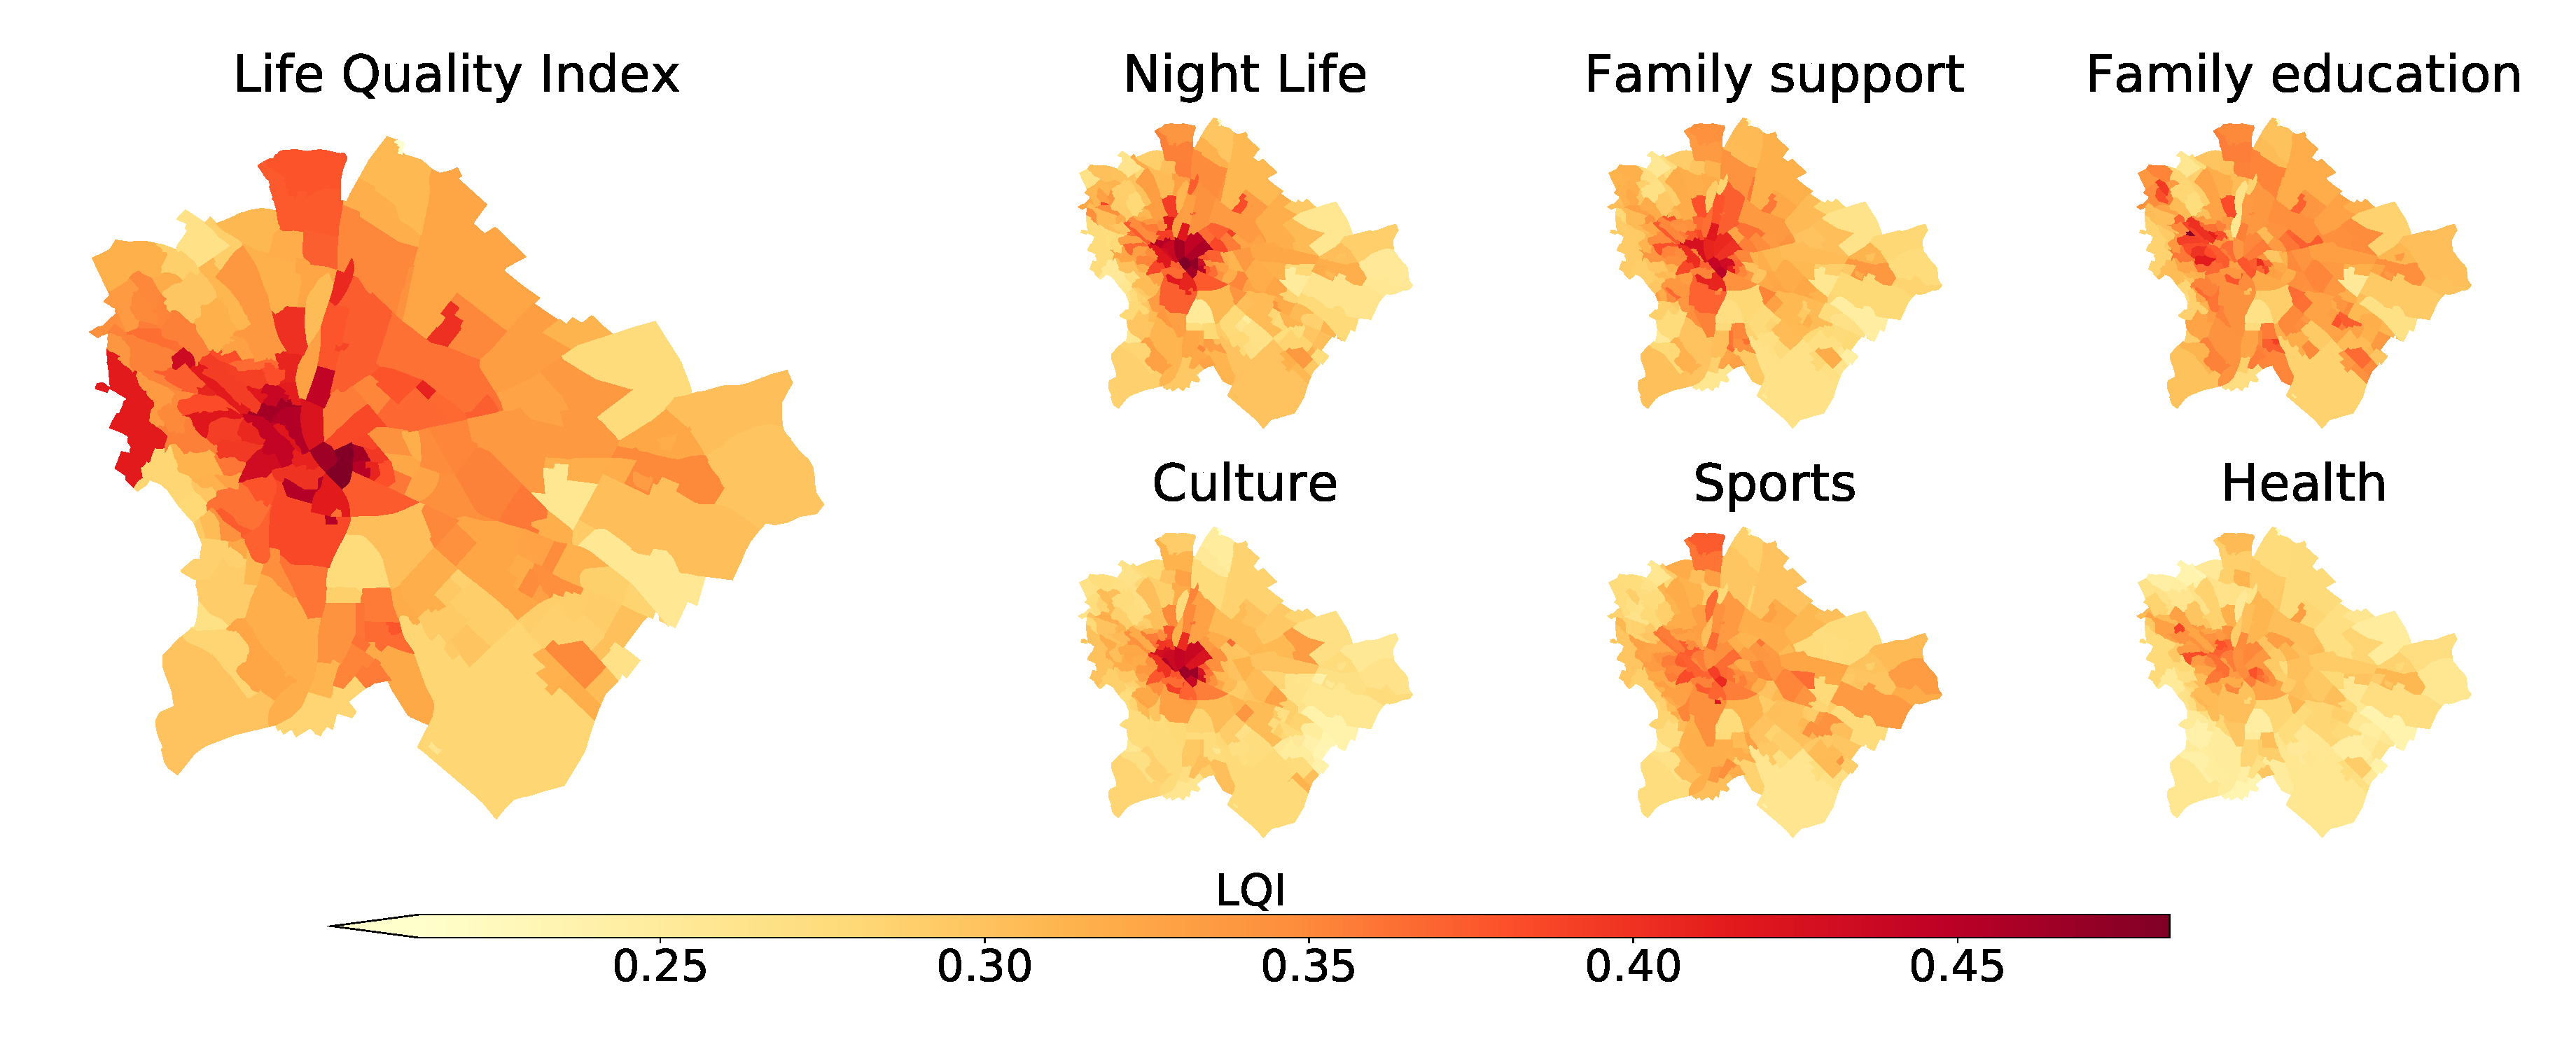
\includegraphics[width=0.8\textwidth]{images/lqi/Budapest_LQI_Neighborhoods-eps-converted-to.pdf}
	\caption[Budapest neighborhoods life quality index]{Budapest neighborhoods, average life quality by categories and aggregated life quality index.}
	\label{fig:BPlqi}
\end{figure*}

Figure~\ref{fig:BPlqi} shows our overall life quality index (LQI) and by categories. Heatmaps reveal important features of Budapest. Similarly to most European cities life quality is much better in the inner districts~\cite{Hohenberg1996Urban,Brueckner1999Central}, especially in the case of Night Life and Culture.

Budapest is divided by the Danube river into two main parts: Buda and Pest. The river does not only serve as a geographical border but due to historical reasons, it also divides the citizens by social status. Hilly Buda, on the West side of the river, used to be the capital of the country, with the residence of the former Hungarian king. On the other side, the mainly flat Pest used to be the agricultural supporter of the aristocrats in Buda~\cite{Kover2006Magyarorszag}. Even though the city has changed dramatically since the Monarchy, the division of Buda and Pest persists, and our life quality index captures it well. However certain services are legally guaranteed to be evenly distributed in the city, such as education and healthcare, for precise modeling one should take into account private care too, which highlights inequalities. So, the traditional division of Buda and Pest is even visible in categories where there should not be that much of a difference (Education, Family Support, Healthcare).

Results also highlight that category LQI-s are highly correlated, less liveable neighborhoods are constant regardless of the amenity category, and well-performing neighborhoods do not change either. It is caused by two main factors: the lack of amenities and the relatively high walking distances in the suburbs.

The compact city concept focuses on building more sustainable and livable cities while designing practical neighborhoods where citizens can maintain everyday life without a car~\cite{Dittmar2012New}. Since, the walkability of a neighborhood highly correlates with its liveability~\cite{Rogers2011Examining} and the suburbs in Budapest do not show any compact city design features, both long distances and the lack of amenities effects suburban habitats lives negatively.

\subsection{Evaluation}

Multiple methods have been developed to evaluate the accuracy of quality of life metrics: Scholars used expert validation with geographic visualization~\cite{Rinner2007Geographic,Gavrilidis2016Urban}, correlations with socioeconomic characteristics~\cite{Talen2002Pedestrian} and surveying citizens’ perceptions of the conditions of life~\cite{Santos2007Monitoring}.

Our evaluation is based on the micro-economical {\it hedonic approach} of estimating the values of public goods. In a capitalist market, real estate prices reflect the recognition of a neighborhood's characteristics: Prices are formed based on demand, more desirable places are more expensive, due to the underlying assumption of providing a higher quality of life.~\cite{Brueckner1999Central} Estimating neighborhoods life-quality with real estate prices has a long tradition in urban literature~\cite{Roback1982Wages,Blomquist1988New,Lora2011New}, therefore we adopt this method to evaluate our model.

We collected the average $m^{2}/EUR$ price for all 23 districts of Budapest in January 2019~\cite{HU2019RealEstate} and correlated each LQI category averaged by district with it. Figure \ref{fig:LQI_ev} shows that our overall LQI correlates the most (R=0.91) with the real-estate prices. Most of its components have a positive correlation with real-estate prices, except the environment which is calculated based on air pollution and green surface proximity. The life quality (LQI) in Budapest is much higher in densely populated downtown districts, which are lack of green surface and suffers from high air pollution due to heavy traffic.

\begin{figure*}[htbp]
	\centering
	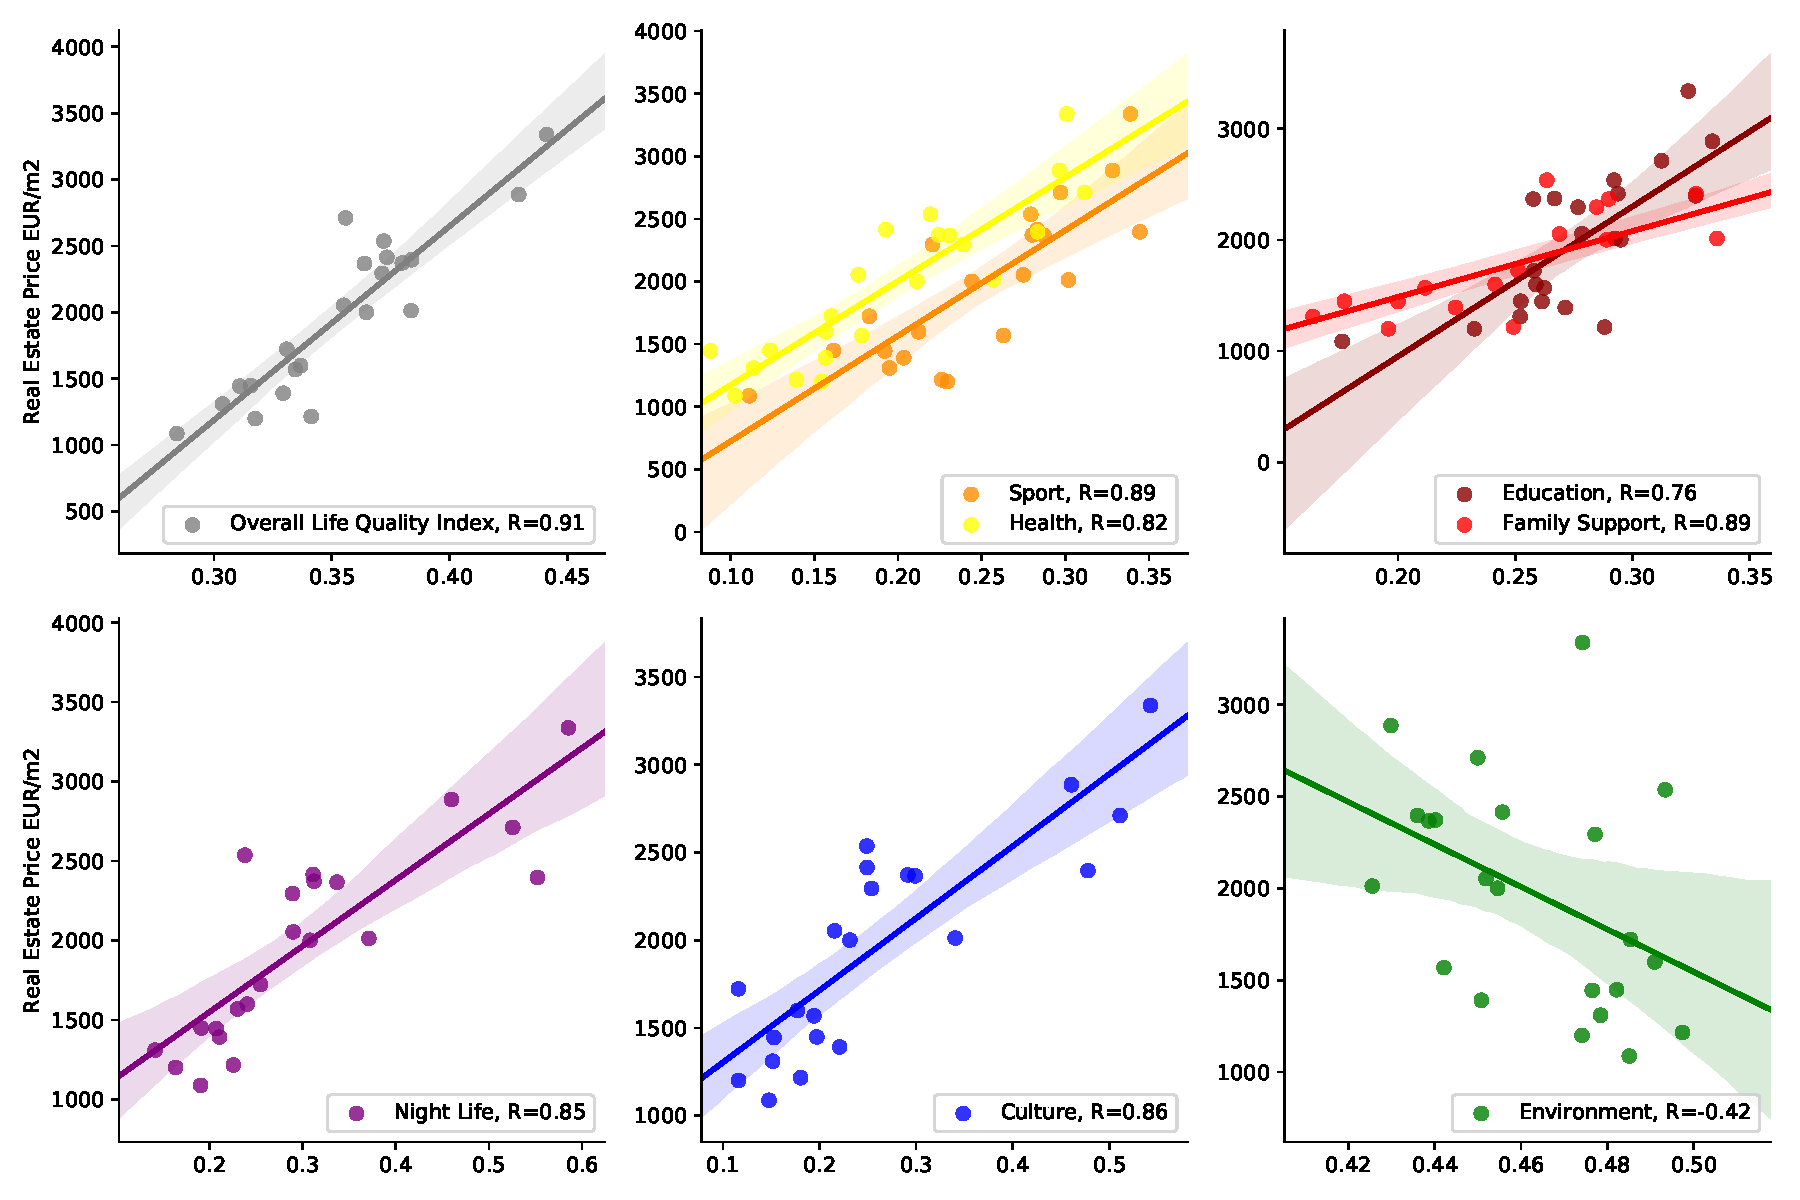
\includegraphics[width=0.8\textwidth]{images/lqi/LQI_categories_regplots.pdf}
	\caption[Budapest life quality index correlation with real estate prices]{Districts of Budapest Life Quality Index (LQI) and its components correlated with real estate prices ($m^{2}/EUR$)}
	\label{fig:LQI_ev}
\end{figure*}

\paragraph{Summary} Locals of Budapest, like in most European cities, traditionally values downtown areas. The relative closeness to CBD, good access to public transport, and vital city life kept it as a desirable area for living~\cite{Cassiers2012Socio}. However, in recent years, the city is facing new challenges: due to gentrification~\cite{Garcia2004Cultural} and over-tourism (eg.:Airbnb) real estate prices are sky-rocketing in downtown areas. In contrast with the early 2000-s when (upper) middle-class moved to the suburbs, nowadays, lower-income families and young professionals are leaving the downtown behind in hope for more affordable living.

As our findings show, Budapest is quite centralized and the quality of life highly correlates with real estate prices, which possibly lead to even more inequalities in the future. This spatial discrimination with longer traveling time, less fulfilling environment, and potential segregation reduces the chances of upward mobility and the quality of life of individuals~\cite{Gobillon2007Mechanisms}.

\section{Discussion}
We have proposed a methodology to quantify life quality as a function of walkability on urban networks. We have used open data to capture inequalities between neighborhoods and districts in the city. We have shown that the real estate market reflects the life quality that our methods found.

A data-driven approach for quantifying life quality at such a granular level like our proposed method can help decision-makers to tackle social and environmental challenges better. Designing compact, liveable neighborhoods, considering also the upcoming environmental crisis is the number one priority of many cities worldwide.

The use of open data sources and algorithmic approaches adds up towards a systematic framework for understanding urban liveability. Our current approach is not the last word in this development since it does not yet account for multiple other variables, such as the quality of services and infrastructure, and other qualitative variables. To capture the more specific indicator of liveability in different cities it would be necessary to work with more granular and city-dependant data.

We anticipate a future stream of research focused on the use of worldwide open data sets to quantify urban liveability, including longitudinal studies in multiple cities, along with algorithmic modeling, simulations, and machine learning approaches, to first quantify the liveability, propose changes and test them with the ground truth data.
\pagestyle{fancy} %LQI walkability
\chapter{Conclusion and open questions}\label{ch:Conclusion}

This thesis set out to contribute to the characterization of multimodal transport infrastructures, develop network science data-driven methods to address the open research problem of planning and identifying strategies to improve sustainable mobility in cities. We leveraged the availability of open high quality urban infrastructure data sets to build the multiplex transportation network of multiple cities. We analyzed the networks first at their multiplex configuration, and later on focused our attention on the bicycle and pedestrian layers.

We started this thesis with a review of previous works on multimodal transportation and mobility research from a complex systems' perspective. In Chapter \ref{ch:litReview}, we covered the science of the dynamics of mobility: How do people move, and which forms of transportation they use? On the other hand these dynamics take place on an underlying (infra)structure which can be modeled by multilayer networks. We offered an overview of mathematical metrics developed in network science recently to the study of the topic. 

After discussing the state-of-the-art research on multimodal mobility and transport infrastructure, we leveraged on the mathematical representation of multilayer transport networks to uncover similarities and differences between multiple cities around the world. The findings presented in Chapter \ref{ch:OverlapCensus} suggest that it is possible to identify and compare those similarities in a systematic and rigorous way using the ``overlap census'' method. These similarities produce clusters of cities with similar multimodal configurations, such as those that have a lack of investment in their sustainable mobility options thus having more car-centric profiles, and clusters of cities with more balanced mobility options.

At the single layer level, we saw in Chapter \ref{ch:BikeGrowth} that a common characteristic of cities is the fragmentation of their bicycle infrastructure networks. We proposed the use of data-driven algorithms to consolidate those components into connected networks to efficiently improve sustainable transport. The two proposed algorithms, when compared with two baselines, highlight the usefulness of growing the bicycle network on a citywide scale (considering all areas of the city) rather than randomly adding bicycle infrastructure. The proposed approach is not the last word in this development, since it does not yet explicitly optimize for directness and does not account for transport flow. As pointed out, the use of data-driven algorithms to identify crucially missing links in bicycle infrastructure has the potential to improve the mobility infrastructure of cities efficiently and economically.

Finally, in Chapter \ref{ch:LQI} we presented a data-driven, network-based method to quantify the liveability of a city based on pedestrian accessibility to amenities and services. We applied the methodology to Budapest and showed that it is able to capture inequalities between neighborhoods and districts in the city. When comparing our findings to average real estate prices we found a positive correlation: the higher the quality of life, the higher the average real estate prices. Our framework demonstrates a way to leverage open data sources to evaluate the quality of life and pedestrian accessibility in systematic city-wide scale.

The literature review (Chapter \ref{ch:litReview}) and the three original chapters (\ref{ch:OverlapCensus}, \ref{ch:BikeGrowth}, \ref{ch:LQI}) directly contribute to the study of multimodal mobility and multilayer transport networks from the network science field. Specifically the literature review is one of the first academic reviews dedicated to covering the topic of multimodal urban mobility and multilayer transport networks from a complexity science perspective.
 
Not only did this research contribute to the growing academic literature, but it also has direct practical application from data-driven policymaking and urban planning perspectives. For instance, the contribution of Chapter \ref{ch:OverlapCensus} on the use of the overlap census to capture similarities among multimodal urban transport networks unravels how different transport modes are interlaced, helping to identify which layer (or set of layers) could be improved to promote multimodal sustainable mobility.

The proposed algorithms and their results in Chapter \ref{ch:BikeGrowth} showed that it is possible to systematically and effectively improve the connectivity of bicycle infrastructure networks. The use of data-driven algorithms to identify crucially missing links in bicycle infrastructure has the potential to help transportation departments and decision makers to improve the mobility infrastructure of cities efficiently and economically. This approach is not only useful for planning urban infrastructures, but could also be used together with  mobility flows simulations to provide insights on how the system will behave after new measures are implemented.

At last, the results presented in Chapter \ref{ch:LQI} highlighted the use of open data and network-based tools to quantify life quality as a function of walkability on urban networks. Such methodology is able to capture urban accessibility inequalities in a detailed manner. A data-driven approach has the potential to help decision-makers tackle social and environmental challenges better. The use of open data sources and the development of algorithmic approaches adds up towards a systematic framework for understanding urban liveability.


\subsection*{Future Work}

The increasing availability of urban and mobility data, together with the continuous growth and developments of computational capabilities and methods are providing us with new research opportunities. For example, data on multimodal mobility, such as digital tickets or wi-fi signals in public transportation, can help to uncover the multimodal mobility dynamics in cities. Furthermore, data sources from share mobility services, as shared bicycles and vehicles, can help us integrate such services with traditional public and private transport infrastructures. Multimodal integration and frameworks are becoming necessary to ensure real-time and user-centered solutions for planning, forecasting and managing services, while increasing safety, and reducing congestion or emissions.

A major challenge for cities will be to integrate and efficiently expand their different multimodal transportation options. The use of data-driven algorithmic approaches for planning bicycle infrastructure networks is one step towards a systematic framework for realistic bicycle network growth strategies. These strategies and algorithmic approaches should consider  qualitative updates, such as integrating planning cultures and processes, along with improving the quantitative methods, for example with the creation of redundant paths that improve the directness and coverage of the bicycle infrastructure. Further research is needed to account for transport flow, and to improve the possibilities for multimodal transport, such as integration with public transport, and the creation of interchange infrastructures.

We have showcased that it is possible to measure the quality of life on urban environments as a function of pedestrian accessibility to amenities. The proposed approach is not the last word on the topic since it does not yet account for other variables, such as the quality of services and infrastructure, along with other variables. Interdisciplinary research efforts will be needed to integrate data-driven algorithmic approaches with qualitative variables. Doing so will let us understand not only the physical aspects that drive the quality of life in cities, but also the qualitative qualities and perceived life quality by their inhabitants.

Understanding cities and their underlying mobility infrastructures is of paramount importance for developing sustainable cities. Indeed, cities and their sustainable mobility infrastructures are one piece in the puzzle towards reversing the global societal threat of climate change. This thesis is our contribution to the understanding of cities, and the development of methods and tools to build a better urban future. \pagestyle{fancy} %Conclusion

% \bibliographystyle{bmc-mathphys}
\bibliographystyle{ieeetr}
\bibliography{bibliography}

\chapter{Appendices}

\section{Life quality as walkability}

\subsection{Secondary data sources}
\label{SI:walkabilityData}
\begin{itemize}
  \item {Sport associations in Budapest}~\cite{HU_sport}
  \item {Kindergartens, daycares, primary and secondary education}~\cite{HU_Edu}
  \item {Art and music schools}~\cite{HU_Art}
  \item {Child health services}~\cite{HU_Child}
  \item {Social welfare system (eg.: elderly care)}~\cite{HU_Social}
  \item{Culture centers}~\cite{HU_Cult}
  \item {Indoor playgrounds}~\cite{HU_Play}
  \item{Healthcare (hospitals, private and public clinics, specialists)}~\cite{HU_Health}
  \item{Fitness and training facilities}~\cite{HU_Fitness}
  \item{Outdoor fitness facilities}~\cite{HU_outfitness}
  \item{Thermal baths and spa}~\cite{HU_Thermal}
  \item{Playgrounds and parks}~\cite{HU_Park}
\end{itemize}

\section{Weights used in the calculations}
The weights of the different $Q$ indices in the final aggregation as well as in sub-categories highly depends on the context and the nature of the problem. Here we present the values we used to generate the results of this study, that were agreed upon consulting with experts.\\
The weights of the sub-indices from equation (\ref{final_Q}) are of the following values:\\
$w^{services}=0.7$\\
$w^{safety}=0.1$\\
$w^{environment}=0.2$\\ \\
The category weights used in equation (\ref{Q_services}), aggregating $Q^{services}$ are:\\
$w^{family}= 0.3$;\\
$w^{health}= 0.3$;\\
$w^{culture} = 0.15$;\\
$w^{sport} = 0.15$;\\
$w^{night life}=0.1$;\\\pagestyle{fancy} %Appendices

% Change list of tables/figures to end
\listoftables
\addcontentsline{toc}{chapter}{List of Tables}

\listoffigures
\addcontentsline{toc}{chapter}{List of Figures}
% until here
\newpage
\backmatter
\afterpage{\blankpage}
\end{document}
